\documentclass[11pt,a4paper]{article}

\usepackage{fullpage}
\usepackage{hyperref}
\usepackage{graphicx}
\usepackage{float}
\usepackage{xcolor}
\usepackage{fancyhdr}
\usepackage{caption}

\setcounter{section}{-1}

\pagestyle{fancy}
\fancyhf{}

\renewcommand{\headrulewidth}{0pt}
\renewcommand{\footrulewidth}{0pt}

\newcommand\instructions[1]{\textcolor{blue}{Instructions: #1}}
\newcommand\todo[1]{\textcolor{red}{TODO: #1}}

%\newcommand\instructions[1]{}
%\newcommand\todo[1]{}

\fancypagestyle{firstpagefooter} {
	\lfoot{\tiny{Version: 17.11.2017}}
	\cfoot{}
	\rfoot{\thepage}
	
}

\lfoot{Name: Gokula Krishnan Santhanam Legi: 16-948-309}
\rfoot{\thepage}

\begin{document}

\title{Advanced Systems Lab Report\\ \normalsize{Autumn Semester 2017}}
\author{Name: Gokula Krishnan Santhanam \\Legi: 16-948-309}
\date{
	\vspace{4cm}
	\textbf{Grading} \\
	\vspace{0.5cm}
	\begin{tabular}{|c|c|}
		\hline  \textbf{Section} & \textbf{Points} \\
		\hline  1                &                 \\ 
		\hline  2                &                 \\ 
		\hline  3                &                 \\ 
		\hline  4                &                 \\ 
		\hline  5                &                 \\ 
		\hline  6                &                 \\ 
		\hline  7                &                 \\ 
		\hline \hline Total      &                 \\
		\hline 
	\end{tabular} 
}
\maketitle
\thispagestyle{firstpagefooter}

\newpage
\section{Report Overview}
This report consists of several sections, going into depth analyzing of the middleware that we have implemented. This sections gives an overview of what to expect in each section and provides a cogent argument as to why the report is structured the way it is structured. Note that this is in no way exhaustive and the corresponding sections will provide more context as well.

We start with describing the system that we built in detail in the \emph{System Overview} section. This goes into the fine-grain details of the design choices we made as well as how the middleware handles the different requests outlined in the project description. 
After this, we first analyze the case when there is no middleware in the \emph{Baseline without Middleware} section, this shows us the throughput and latency trends when there is no middleware and also gives a sense of the limits of the memtier clients and memcached servers. We also analyze the bottlenecks in this section.

Now, we introduce the Middleware in \emph{Baseline with Middleware} and repeat similar experiments to understand the limits of the middleware as well as how the throughput and response time trends change as a result of introducing the middleware. We further analyze the bottlenecks in this setup.

In the middleware, we handle SETs, GETs and multi-GETs different and would like to know how exactly the trends in throughput and latencies vary for these different kinds of requests. Especially because we replicate in the case of SETs and might do sharding in the case of multi-GETs. We analyze the trends for these different types of requests in the \emph{Throughput for SETs} and \emph{Gets and Multi-gets} sections respectively.

In our experiments with memtier clients, memcached servers and middlewares, we can fundamentally change a few properties. These are the number of virtual clients per thread at the load generating VMs, the number of middlewares in place and the number of worker threads per middleware. We analyze how sensitive the throughput and latency is to these parameters by conducting a 2k analysis in the \emph{2K Analysis} section. 

Finally, we model our system in accordance to queueing theory and see how well the things we observe correspond to theory in the final section, \emph{Queuing Model}.

Several appendices are also provided which delve into more details.


\section{System Overview} % DONE, need to revise
%\instructions{Describe the implementation of your system and highlight design decisions relevant for the experiments. Explain how messages are parsed and how statistics are gathered in a multi-threaded setting. Provide figures containing all the threads and queues in your system (including the network and the memcached servers). Include illustrations that show how requests of different types are handled (e.g., components involved in processing the request and method calls). Please include all details necessary to understand artifacts and effects in your experiments that arise from your implementation choices.}

The three main components of the middleware are
\begin{itemize}
	  \setlength{\itemsep}{0pt}
	  \setlength{\parskip}{0pt}
	  \setlength{\parsep}{0pt}
	\item Net Thread / frontend  (\texttt{MyMiddleware.java})
	\item Request Queue and Request object (\texttt{Request.java})
	\item Worker Threads / backend (\texttt{Worker.java})
\end{itemize}

In addition to the above three, there is another class \texttt{utils.java} which is used to provide methods to handle parsing and other auxiliary methods which will be discussed in a later section. This enables a modular design and makes the code less error prone. Loggers are added to both the Net and Worker threads in order to log any errors and other information. More details about the instrumentation are discussed in a later section as well. Before processing these logs, the error logs are checked to make sure no errors occurred before proceeding further with the analysis. This ensures that the data used in the subsequent analyses is sane and the results are meaningful. 

All the code for the middleware are under the \texttt{src} directory in the project’s repository. The scripts used to postprocess the logs are in the \texttt{scripts} directory. More information about each script can be obtained from the \texttt{README} files in the same directory. The logs are stored in the \texttt{logs} directory.

All code has been extensively documented and tested with experiments repeated to make sure that no bugs had creeped into the middleware and that variations due to the VM allocation in the cloud did not severely the measurements. All logs like mentioned above were checked before being included in the analysis. This is true of logs generated by both Middleware and Memcached.

A simple graphical representation of the middleware is shown below.
	\begin{figure}[h]
		\caption{Components of the middleware}
		\centering
		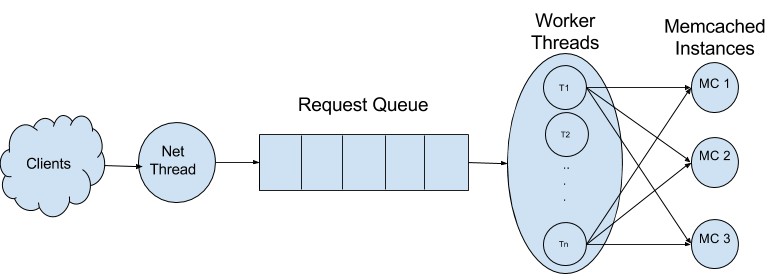
\includegraphics[scale=0.525]{images/1_MW_simple.png}
	\end{figure}

\subsection{Net Thread}

	The Net Thread is the entry-point into the middleware and is created by the \texttt{RunMW.java} script. In its constructor, the net thread creates the request queue and also creates an appropriate number of worker threads with the arguments it is given.
Once these are created, the net thread then creates a non-blocking \texttt{ServerSocketChannel} to listen to new connections. This and any new connections that are established are put into a \texttt{Selector} and polled. The Selector enables us to handle multiple connections efficiently using just a single thread. Both the \texttt{ServerSocketChannel} and \texttt{SocketChannel}s corresponding to the established connections are configured to be non-blocking in order to make full use of the Non-Blocking IO facilities provided by Java. The \texttt{ServerSocketChannel} is registered with \texttt{OP\_ACCEPT} and the \texttt{SocketChannel}s are registered with \texttt{OP\_READ} SelectionKeys in order to be notified when there are new connections and when there is data to be read on the connection respectively.  This way, we use only one selector to handle a ServerSocket channel and N SocketChannels (where N is the number of clients connected to the middleware). Any time a connection is closed, it is removed from the selector. When a connection is closed, it is selected by the selector and when \texttt{read} is called on the socket channel, we read back \emph{-1} bytes indicating that the channel was closed by the remote peer (the Virtual Client on the memcached instance).


The Net thread blocks on calling \texttt{select} of the Selector, which returns only when one of the registered channels have a new connection or some data to be read. Thus, the net thread does not do busy waiting. Whenever there's a new connection, we obtain the socket channel corresponding to that connection by calling \texttt{accept} on the ServerSocketChannel and add it to the selector. This is handled by the \texttt{addNewConnection} method of the Net thread.


Whenever there's incoming data in the established connections, we create a \texttt{ByteBuffer} instance of appropriate size and write into it. We then check if the message is complete (using \texttt{utils.isCompleteRequest}) by counting the number of new-lines in the received request. The request is complete if there are one and two new-lines in the case of \texttt{GET} (also \texttt{multi-GET}) and \texttt{SET} request respectively.


If the request is not complete, we attach the byte buffer to the SelectionKey (using the \texttt{.attach} method)and continue processing other requests. This allows the middleware to not wait for one client to send a complete request before processing other clients.The next time there is new data in the same channel, the attached byte buffer is used instead of creating a new one. We check for completion every time we read from a socket channel.


When the request is complete, we create a new \texttt{Request} object with the byte buffer and the corresponding socket channel and add it to the request queue. the above workflow of handling data in established connections is handled by the \texttt{readRequest} method.


Every time we add a new request to the request queue, we log the current length of the queue in a separate logger.

\subsection{Request Queue}
	The request queue is an instance of the \texttt{LinkedBlockingQueue<Request>} class. It contains instances of the \texttt{Request} class which encapsulate all the relevant information about a request as it passes through the middleware. We use this particular class due to several performance and design reasons which we elaborate in this section.


First, LinkedBlockingQueues are unbounded, this means that they can grow indefinitely (subject to total memory available, of course). Due to this unboundedness, we are assured that no request that arrives to the middleware is dropped and thus makes our later analysis simpler. 


Second, the LinkedBlockingQueue is thread safe, which means that multiple worker threads can safely dequeue from it and we don’t have to implement any complicated synchronization routines to ensure data integrity. 


Finally, It also allows worker threads to block on it when there are no requests available for them to process (hence the name \texttt{LinkedBlockingQueue}). This prevents busy waiting and the resultant wasting of CPU clock cycles thereby improving the utilization of resources available at the middleware. Moreover, it can wake up exactly one worker thread blocking on it when there’s a new request (internally it uses \texttt{notify} and not \texttt{notifyAll}) thus preventing the thundering herd problem that occurs when multiple threads sleep on a single resource.


As we just saw, the \texttt{LinkedBlockingQueue} satisfies all the design and performance requirements we need of a request queue in the middleware and was chosen as a result.

\subsection{Worker Threads}
The worker threads do a majority of the tasks inside the middleware. These are started by the Net Thread during initialization. Each worker thread is given the following information as arguments to its constructor.
\begin{enumerate}
	  \setlength{\itemsep}{0pt}
	  \setlength{\parskip}{0pt}
	  \setlength{\parsep}{0pt}
	\item List of Memcached IP and Ports
	\item A Reference to the Request Queue
	\item Boolean flag (sharded or non-sharded mode)
	\item Worker ID and logging directory 
\end{enumerate}
The Worker ID is used to uniquely identify a thread among all worker threads. This, along with the logging directory allows the thread to store its information in an uniquely named log file.

Inside the constructor, the worker thread creates a connection to each of the Memcached instances and adds the socket channels to an \texttt{ArrayList}. 
Each worker thread creates a blocking socket channel to each one of the memcached servers. resulting in num\textunderscore worker\textunderscore thread * num\textunderscore memcached\textunderscore servers connections in total.  

These socket channels are configured to be blocking because our worker threads are synchronous and handle only one request at a time. Nevertheless, We still use the socket channel because it provides for an unified interface at both the Net thread and the Worker thread and makes the implementation easier and less error prone as you only need to pass byte buffers around. The worker thread also creates loggers to log information about the requests it processes and any errors that it may encounter during an experiment. Once again, these logs are checked (after the experiment is completed) before running any analysis on them to ensure that we are working with logs which have meaningful data and that our experiments did not run into any errors or unusual behaviours.

In the \texttt{run} method, the worker threads block on \texttt{requestQueue.take} until is woken up by a new request in the queue. The worker thread dequeues it and calls \texttt{processRequest} to handle it. All the information about the current request is logged once the control return backs from the \texttt{processRequest} method.

processRequest inspects the request to check if it is a \texttt{GET} or \texttt{SET} and passes it along to \texttt{processGetRequest} and \texttt{processSetRequest} accordingly.

The life-time of a request inside the middleware is shown in the graphic below. Here, MC refers to the memcached servers.
	\begin{figure}
		\caption{Life of a request inside the middleware}
		\centering
		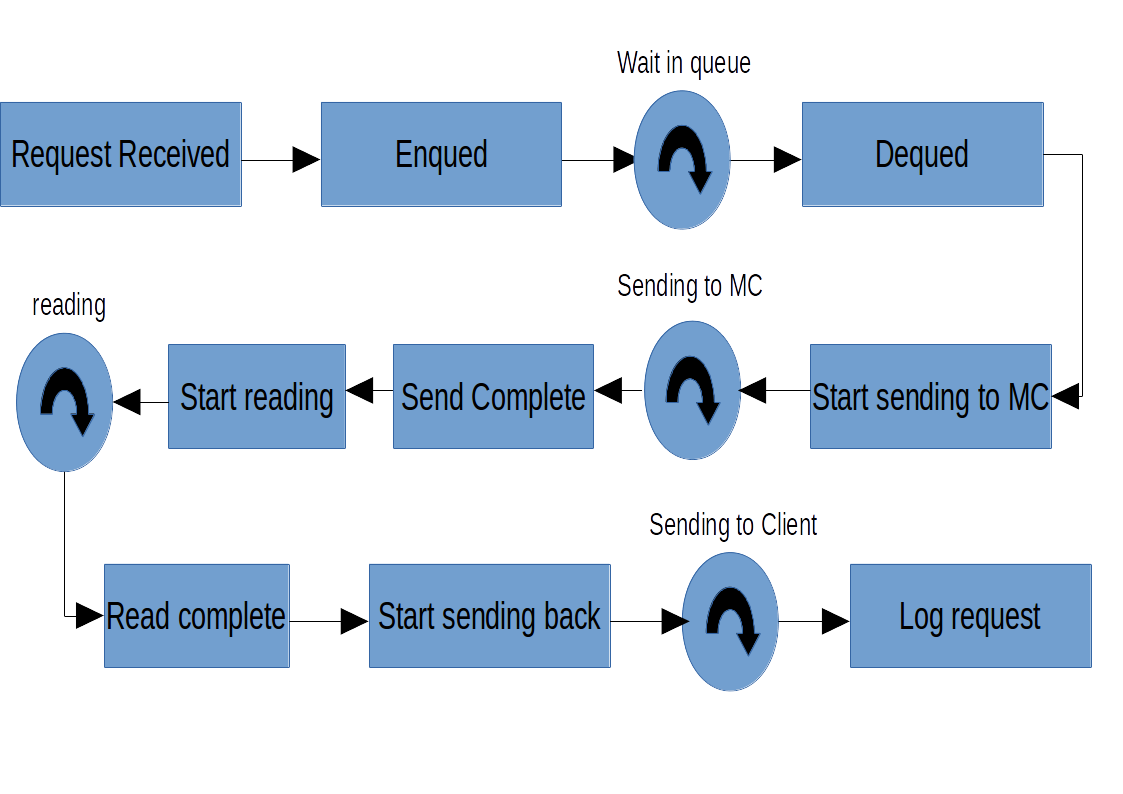
\includegraphics[scale=0.5]{images/1_life-of-a-request.png}
	\end{figure}


	\subsubsection{Handling SET Requests}
	\texttt{SET} requests are handled by the \texttt{processSetRequest} method. This method iterates through the list of socket channels and sends the request to each of the memcached instances sequentially. After sending to a server, byteBuffer.rewind is called to reset the position of the bytebuffer to zero. This allows us to use the same bytebuffer for each one of the memcached servers and no new copies are created. The responses are read back only after sending to all the servers. We log \texttt{timeStartSendToMC} when we start sending the requests. We also log \texttt{timeSentToMC} when we are done sending the request to each of the servers.
	
	Once the request is forwarded to the memcached servers, we allocate a new byte buffer and iterate through the socket channels again to read in the responses. We log \texttt{timeStartRecvdFromMC} before starting this process. If the response is not \texttt{STORED\textbackslash r\textbackslash n}, then a copy of the response is added to a list of exceptions and the buffer is cleared before moving to the next memcached instance. \texttt{timeFinishedRecvdFromMC} is logged once we finish reading from each of the servers.
	
	After reading all the responses, we check if the list of exceptions is empty or not. If it is not empty, the first response is taken and returned back to the client through the request's socket channel. All exceptions are logged even though only one is sent back to the client.
	
	If the exceptions list is empty,  the SETs have succeeded. We reuse the contents of the buffer we use to read back the responses (which will be having \texttt{STORED \textbackslash r \textbackslash n} in this case) and send it back to the client.
	
	\subsubsection{Handling GET requests}
	Handling GET requests is more complicated because of the number of different ways we need to process them. As a result, we have the following program flow.  As soon as we detect that the request is a \texttt{GET}, we hand it over to \texttt{processGetRequest} method. The \texttt{processGetRequest} first checks if the request is a single or a multi-\texttt{GET} by counting the number of "spaces" in the request. If there is more than one space in the request, it's a multi-GET. The request is then handed off to one of \texttt{processSingleGetRequest} or \texttt{processMultiGetRequest} respectively. 
	
	\paragraph{i. Handling Single GETs}
	The \texttt{processSingleGetRequest} method is straight-forward and easy to understand. It simply forwards the request to one of the memcached servers and reads back the response. The timestamps \texttt{timeStartSendToMC} is recorded before sending the request to memcached and \texttt{timeSentToMC} is recorded after sending the request to the memcached server.
	
	In order to ensure that each of the memcached servers experience equal amounts of load from the single-GET requests, we use a variable called \texttt{whosNext} which keeps track of which memcached server to forward the request to. \texttt{whosNext} is incremented (and modulo number of memcached servers) after every request. There is one instance of this variable per worker thread and allows us to use a round-robin scheduling to assign single GET requests to memcached servers.
	
	We use the \texttt{isCompleteResponse} method from the utils class to check if we have got the entire response back from the memcached server. We keep reading from the server in a while-loop until we have the entire response. This completeness check is especially important in the case of multi-GETs without sharding where the response can become very large and we may not get the entire response in one single \texttt{read} call.
	
	The timestamps \texttt{timeStartRecvdFromMC} and \texttt{timeRecvdFromMC} are recorded before we start reading and after we finish reading respectively.
	
	Once the complete response is with the middleware, the method then checks if the response starts with \texttt{VAL} or \texttt{END}. These correspond to the case when we found the key in the memcached server and it has returned back the value and the case when we have a GET miss respectively. Note that the latter case will never happen due to the fact that we pre-populate the memcached servers with all the keys we use. Nevertheless, we handle the GET misses case as well. If the response is neither of these, then it is an error and the entire request and response is logged. After this, the worker thread moves on to process the next request available in the queue.
	
	In case that all sanity checks pass, and we have a valid response, the method simply flips the buffer and forwards the response back to the client. The timestamps \texttt{timeStartSentBack} and \texttt{timeSentBack} are recorded before starting and after completing the \texttt{socketChannel.write} call. 
	
	\paragraph{ii. Handling Multi-GETs}
	Handling multi-GETs is a bit tricky due to the multiple sub-cases that arise. Inside the \texttt{processMultiGetRequest}, we first check if the \texttt{isSharded} flag is set. This flag corresponds to whether we need to shard the multi-GET request or not. We also check if the number of memcached servers is greater than one. If either of the above conditions is not true, then the multi-GET request can be treated as a single-GET request and so the \texttt{processSingleGetRequest} is called with the request. Therefore, \texttt{processMultiGetRequest} is used if and only if the sharded-mode is enabled and there are more than one memcached servers.
	
	If the above conditions are satisfied, we first split the received request into shards. This is done by \texttt{utils.getShards} method which gives us as many shards as there are memcached servers. The method extracts the keys from the multi-GET request and creates the shards from the bottom up in a round-robin fashion by looping across the shards and appending one key at a time until there are no keys left in the multi-GET request.
	This way, we can guarantee that the sharded requests are of almost equal size. They become slightly unequal when the number of keys is not divisible by the number of memcached servers. In such cases, some of the shards have one key extra. No sharding technique can circumvent this issue because it is mathematically impossible to equally divide the load when the number of keys is not a multiple of number of memcached servers.
	
	Note that in our experiments, we always have situations where the number of keys in a multi-GET request is divisible by the number of memcached servers so we can assume that the shards are always of equal size in practice. As a result, each multi-GET request puts equal load on each of the memcached servers.
	
	Once we have the shards, we send one shard per memcached server and log the \texttt{timeStartSendToMC} and \texttt{timeSentToMC} before and after we send the requests.
	
	After this, we read back the responses from each of the memcached servers (checking if we have got the complete response) and store them in an array list. We also log \texttt{timeStartRecvdFromMC} and \texttt{timeRecvdFromMC} before and after we receive all the responses. 
	
	We also check if the responses start with "VAL" or "END" to ensure that we don't get any errors. If there are any, we log them separately and move onto the next request in the queue.
	
	The arraylist of responses is sent to \texttt{utils.joinShards} which combines the responses into one. It does this by iterating through the responses, stripping off the "END\textbackslash r \textbackslash n" at the end of each response and appending the responses together. It finally appends a "END\textbackslash r \textbackslash n" at the end of the combined response to make it a valid response to a multi-GET request.  
	
	This is then sent back to the client as the response to its request. We log the \texttt{timeStartSentBack} and \texttt{timeSentBack} timestamps before and after sending the request back.
	
	Once the logic returns back from either \texttt{processSetRequest} or \texttt{processGetRequest}, we log to disk all the timestamps corresponding to the request that was processed before moving on to process the next request in the queue (if any). 
	
	The flow-chart in the next page illustrates the logic flow of handling requests inside the worker thread.


\subsection{Request Object}
The request object follows from the Object Oriented Programming (OOP) paradigm and provides encapsulation to keep all the information about a particular request in one place. This includes the socket channel corresponding to the connection from which the request came from as well as the byte buffer that contains the actual contents of the request.

Along with the above two, the request object 	has timestamps (in nanoseconds, obtained using \texttt{System.nanoTime}) for each event in the life of a request in the MW. These include
\begin{itemize}
	  \setlength{\itemsep}{0pt}
	  \setlength{\parskip}{0pt}
	  \setlength{\parsep}{0pt}
	\item \texttt{timeCreated} When the request was created
	\item \texttt{timeEnqueued} When the request enqueued
	\item \texttt{timeDequeued} When it was dequeued
	\item \texttt{timeStartSendToMC} When we start sending to memcached servers
	\item \texttt{timeSentToMC} When we finish sending
	\item \texttt{timeStartRecvdFromMC} When we start reading back responses
	\item \texttt{timeRecvdFromMC} When we finish reading responses
	\item \texttt{timeStartSentBack} When we start sending back response to client 
	\item \texttt{timeSentBack} When we finish sending back response
\end{itemize}
It also has which type of request it is (SET or GET) in \texttt{reqType} attribute. \\


Finally, the Request object also has a \texttt{GetLoggerLine} method for formatting the timestamps into a line to log in the info logs.

\subsection{utils}
The utils class contains several auxiliary methods that are used to process the contents received in the byteBuffers. We keep these methods separate from the classes themselves so that their functionality can be used across classes and makes debugging and testing these methods easier. This also provides for a cleaner codebase as well. All the methods in this class are static so that you don’t need to instantiate an object of this class to use them.  Most of these methods receive a bytebuffer as an input and do not create copies of bytebuffer explicitly or implicitly  (by creating new String objects). Instead, they obtain a view into the underlying byte array to handle the processing thereby saving memory and reducing performance overheads.

	The methods in this class include
	\begin{itemize}
		\setlength{\itemsep}{0pt}
		\setlength{\parskip}{0pt}
		\setlength{\parsep}{0pt}
		\item \texttt{getRequestType} checks if request is a GET or SET or something else
		\item \texttt{isSingleGet} checks if a GET request is single or multi-GET
		\item \texttt{countNewLines} counts the number of "/r/n" in the byte buffer
		\item \texttt{isCompleteRequest} checks if we have complete request from memtier clients
		\item \texttt{isCompleteResponse} checks if we have complete response from memcached servers
		\item \texttt{getShards} shards a single multi-GET request into multiple smaller multi-GETs when using the middleware in sharded mode
		\item \texttt{joinShards} combines responses for each shard (smaller multi-GET) sent to memcached servers while the middleware is used in sharded mode. joinShards helps combine multiple responses into one which is sent back to the client.
	\end{itemize}
	
	\subsection{Logging Infrastructure}
	Logging plays an important part in the middleware as the logs are important for all the analysis we do downstream. There are multiple log files that are generated by the middleware. All log files that contain errors end with a \texttt{.error} suffix and those that information (like that of a request) end with \texttt{.info} suffix. Additionally, we log the queue lengths separately in a file with \texttt{.length} suffix.
%	\pagebreak
	\begin{figure}[H]
		\caption{Logic Flow of handling requests in the worker thread}
		\centering
		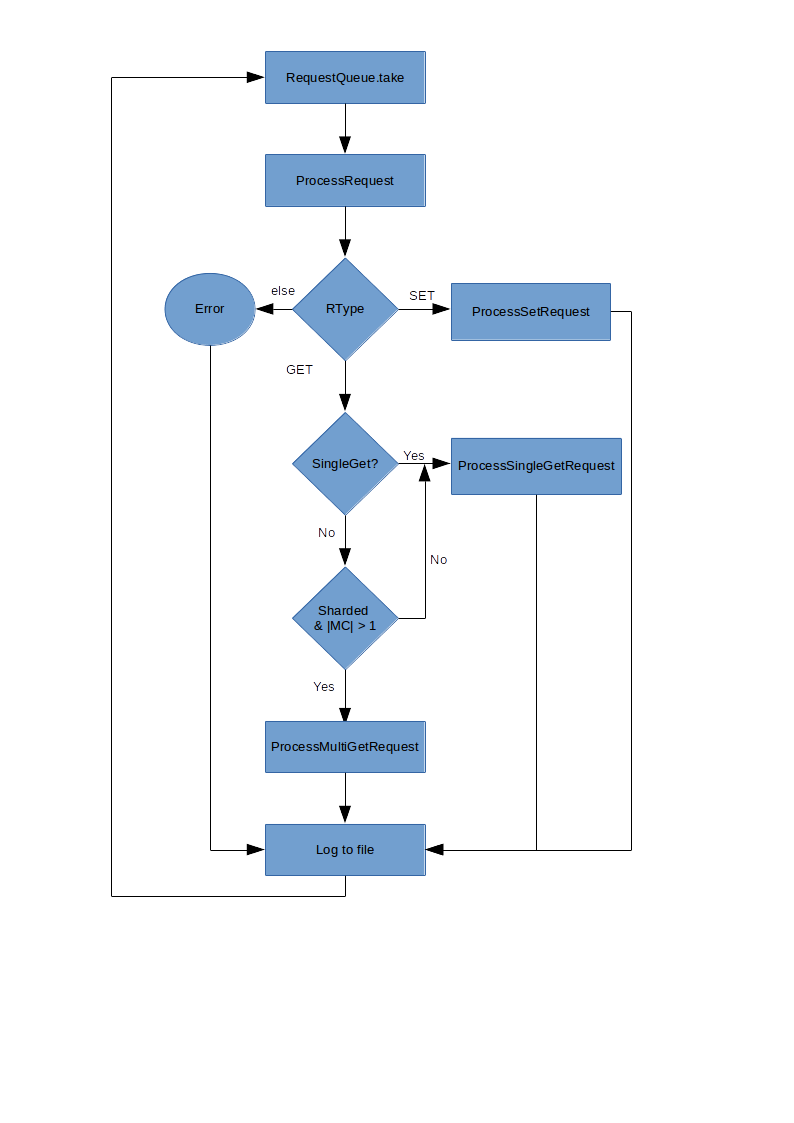
\includegraphics[scale=0.9]{images/1_worker_logic_flow.png}
	\end{figure}
	%\pagebreak	

	

	
	The Net thread and each of the worker threads generate their own log files and have the following naming convention.
	
	\texttt{mc-<num\textunderscore memcached\textunderscore servers>\textunderscore workers-<num\textunderscore worker\textunderscore threads>\textunderscore shard-<sharding\textunderscore flag>\textunderscore }
	If the log files are from the frontend, there's a \texttt{frontend} appended to the convention above. \texttt{id\textunderscore <worker\textunderscore thread\textunderscore id>} is appended if the files are from a worker thread.
	
	An example would be \texttt{mc-3\textunderscore workers-64\textunderscore shard-false\textunderscore id-0.info} which corresponds to the configuration when there are three memcached servers, 64 worker threads, sharding disabled and the file is the INFO logs of the first worker thread (id-0). As mentioned earlier, log files are sanity checked before being used in the analysis downstream. This is done using \texttt{scripts/raw\textunderscore mw\textunderscore sanity\textunderscore check.py} script. The sanity check involves making sure that all the ERROR files are empty and that none of the INFO files from the workers are empty. These two conditions ensure that the middleware operated nominally during our experiments.
	
	We do similar sanity checks with the memtier generated logs using the \\ \texttt{scripts/mt\textunderscore sanity\textunderscore check.py} script. Sanity checks here implies checking that the JSON file is parsable, that there are no GET misses and that the response times are not infinity.
	
	We log information about each request (all timestamps and request type mentioned in the section about the Request object), this enables us to have much finer analysis of the middleware’s performance and obtain deeper insights about the middleware’s performance like if the garbage collector significantly affected performance at some time or not (it did not). We don’t write to disk immediately after each request completes but buffer our writes. This way, we save a large amount of unnecessary I/O operations and as a result the middleware performance is not adversely affected. It is also interesting to note that logging every request is not unusual even in production environment. In fact, the Apache webserver logs every single HTTP request it gets.
	
	Finally, we use the \texttt{scripts/mw\textunderscore folder\textunderscore postprocessor.py} script to aggregate information like throughput and response time across the worker threads for further analysis.
	
	\subsection{Load Distribution Among Memcached Servers}
	
	Due to the round-robin scheduling we exploit, each worker thread distributes its single-GETs load equally to each memcached server. The SETs are naturally equally distributed because they are forwarded to each of the memcached servers. The only remaining request type is multi-GET and the mechanism by which we equally distribute multi-GET requests among the memcached servers (in both sharded and non-sharded modes) has been discussed in the previous sections.
	Thus, each worker thread distributes its load equally among the memcached servers, and we can extend this to say that the middleware distributes its load equally among all the memcached servers. 



\section{Baseline without Middleware} % TODO

\underline{\textbf{NOTE}} It is highly recommended to read the appendix \ref{appendix_a} \emph{General Notes on Experimental Setup} to get the common setup which applies across all the experiments.

%In these experiments we study the performance characteristics of the memtier clients and memcached servers. In the first part, where there is only one memcached server, we increase the number of virtual clients from the load generators. In the second set of experiments, there are now two MC servers and only one Load Generating VM with two instances of memtier, one connecting to each of the memcached server. For the first set of experiments, the hypothesis is that we are pushing the MC server to its limit in order to find its maximum throughput i.e., we assume that the memcached server is the bottleneck and find out the maximum throughput it can handle. In the second set of experiments, the load generating VMs and consequently, the memtier instances are assumed to be the bottleneck and we try to find out what's the maximum throughput a single memtier instance can deliver to the MC servers. These two numbers are assumed to form natural upper-bounds to the maximum throughputs we can expect from the middleware in later sections. This is because the middleware is assumed to be the slowest of the three components and will be the bottleneck.

%It is important to note that the above statements are hypotheses we are testing in this section and may turn out to be incorrect. In such cases, a logical explanation backed by data would be provided and a coherent view of the system under analysis would be reached.

\subsection{One Server}

%\instructions{Both, for a read-only and write-only workload plot the throughput and the response time as a function of NumClients. All clients are connected to a single memcached instance.}

%\instructions{Use 3 load generating VMs, with one memtier (CT=2) each, and vary the number of virtual clients (VC) per memtier thread between 1 and 32. Show how the behavior of the server changes as we add more clients.}



\subsubsection{Commands}
The following are the commands used to start the memtier instances and memcached instances
{\scriptsize{memcached instance: \texttt{memcached -t 1 -p 6969} \\
memtier instance: \\
For Write-Only Workloads: 
						 \texttt{memtier\_benchmark -s <MC\_IP> -p 6969 -P memcache\_text -t 2 -c <NUM\_VC\_PER\_THREAD> \\ --ratio 1:0 --test-time 80 --json-out-file <LOG\_FILE> } \\
For Read-Only Workloads: 
						 \texttt{memtier\_benchmark -s <MC\_IP> -p 6969 -P memcache\_text -t 2 -c <NUM\_VC\_PER\_THREAD> \\ --ratio 0:1 --test-time 80 --json-out-file <LOG\_FILE> } }} \\
The naming conventions used are explained in the relevant sections in the report as well as in the \texttt{logs/} directory of the repository. \texttt{<MC\_IP>} is the private IP of the memcached server (In the 10.0.0.x range)

\subsubsection{Experimental Configuration}
\begin{center}
	\scriptsize{
		Experiment Configuration for One Server baseline Experiments
		\begin{tabular}{|l|c|}
			\hline Number of servers                & 1                        \\ 
			\hline Number of client machines        & 3                        \\ 
			\hline Instances of memtier per machine & 1                        \\ 
			\hline Threads per memtier instance     & 2                        \\
			\hline Virtual clients per thread       & [5, 15, ..., 145]        \\ 
			\hline Workload                         & Write-only and Read-only \\
			\hline Multi-Get behaviour               & N/A                      \\
			\hline Multi-Get size                   & N/A                      \\
			\hline Number of middlewares            & N/A                      \\
			\hline Worker threads per middleware    & N/A                      \\
			\hline Repetitions                      & 3 (1 minute steady state)\\ 
			\hline 
		\end{tabular}
	} 
\end{center}

\subsubsection{Plots}

\begin{figure}[H]
	\captionsetup{font=scriptsize,labelfont=scriptsize,justification=centering}
	\centering
	\begin{minipage}{0.5\textwidth}
		\centering
		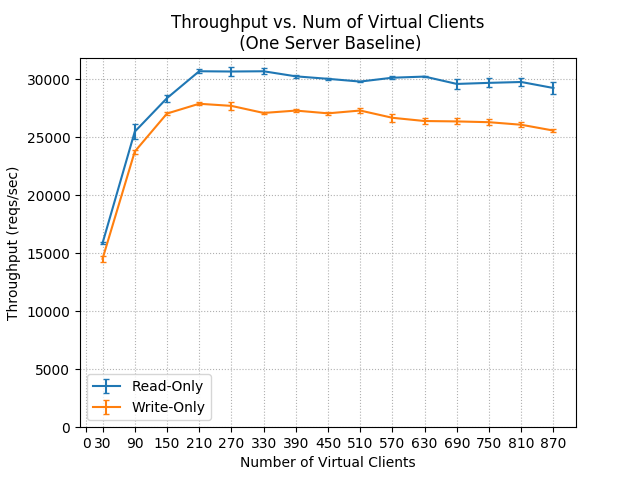
\includegraphics[scale=0.525]{images/2a_one_mc_tps.png}
		\caption{Average Throughput for baseline without middleware,\\ one memcached server}
		\label{tps_1_mc_baseline}
	\end{minipage}\hfill
	\begin{minipage}{0.5\textwidth}
		\centering
		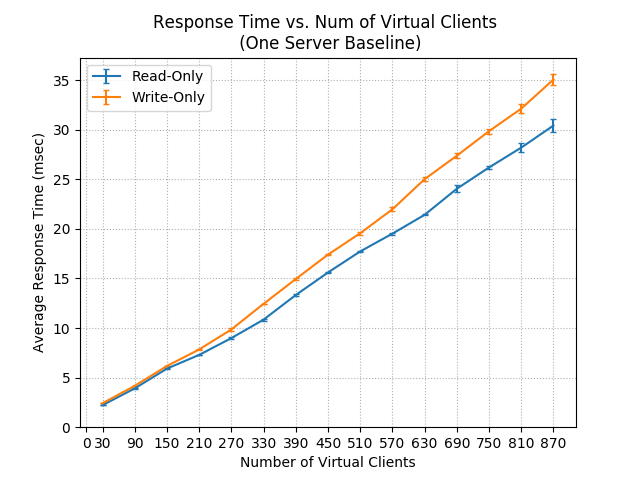
\includegraphics[scale=0.525]{images/2a_one_mc_rt.png}
		\caption{Average Response Time for baseline without middleware,\\ one memcached server}
		\label{rt_1_mc_baseline}
	\end{minipage}
\end{figure}

\subsubsection{Explanation}
% \instructions{Describe in which phase the memcached servers are under-saturated, saturated, or over-saturated. Describe how throughput and response time correlate. Explain what further conclusions can be drawn from the experiment.}

From the throughputs plotted in Figure.\ref{tps_1_mc_baseline}, we can see that for the read-only and write-only loads, the throughput flattens out at around 210 virtual clients. Thus, we can say that the memcached server is under-saturated when the load is less than 210 virtual clients and saturated beyond that. Memtier clients wait for a response before sending the next request, hence the number of requests in the system (memcached + memtier) is bounded. Thus, we can say that the system is closed and as a result, we don't see the oversaturation phase. The errors in measurement are nominal and thus we can conclude that the network, MC servers and MW clients were all stable during our experiments.

From both the plots, we can see that for a given number of virtual clients, the writes have lower throughput and higher response times. From the memcached protocol, we can see that the number of bytes in a SET request are higher than those in a GET request (the SETs have to contain the value to be stored along with the key). This trend is reversed if we consider the response, i.e., responses to GETs are bigger than responses to SETs. 

It more instructive to discuss the bottlenecks after we discuss trends with the two server experiments and are able to compare the trends observed in both.

The Interactive law connects the throughput (X) and the response time (X) of a system. This can be written as 
$ R = N / X - Z$. Here, Z is the thinking time for the clients. In most cases, including ours, this is assumed to be zero. Thus, the law simplifies to $ R = N / X$. N is the number of jobs in the system, in this case, the number of virtual clients.

We plot the response time vs. throughput plot for the one memcached experiments below. The plot verifies that our observations follow the interactive law (within error bounds).
\begin{figure}[H]
	\captionsetup{font=scriptsize,labelfont=scriptsize,justification=centering}
	\centering
		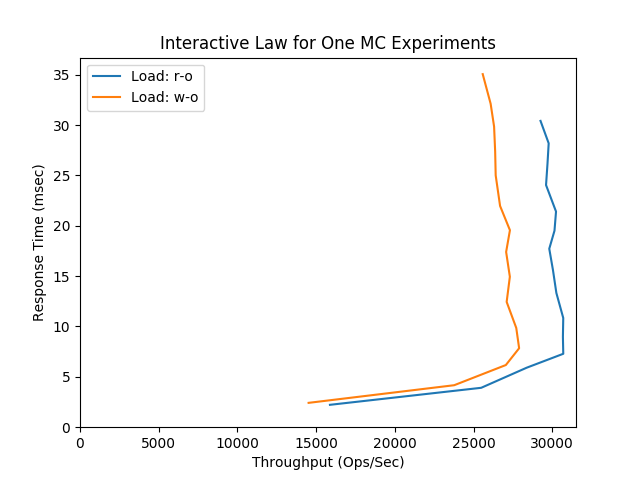
\includegraphics[scale=0.7]{images/2a_interactive_law.png}
		\caption{Interactive Law Plot, one memcached server}
\end{figure}

%\todo{
%Also, talk about why the tps for gets is higher than for sets (due to network / buffer at MC effects?). Consider the fact 
%that this trend is reversed in the next section. \\
%Similarly, talk about why the response time for sets is higher, it is flipped. \\
%\textbf{Which component is the bottleneck? Why?} } 

%\todo{
%What further conclusions can you draw? When is MT bottleneck and when MC is bottleneck? \\
%Also,verify the interactive law for a few points.
%write down the interactive law as well.
%}


\subsection{Two Servers}

%\instructions{For a read-only and write-only workload plot throughput and response time as a function of NumClients. The clients are connected to two memcached instances.} 

%\instructions{Use 1 load generating VM, with one memtier (CT=1) connected to each memcached instance (two memcache instances in total), and vary the number of virtual clients (VC) per memtier thread between 1 and 32. Show how the behavior of the server changes and explain what conclusions we can draw from this experiment.}

\subsubsection{Commands}
The following are the commands used to start the memtier instances and memcached instances
{\scriptsize memcached instance: \texttt{memcached -t 1 -p 6969} \\
memtier instances:\\
For Write-Only Workloads: \texttt{memtier\_benchmark -s <MC\_IP\_1> -p 6969 -P memcache\_text -t 1 -c <NUM\_VC\_PER\_THREAD> --ratio 1:0 --test-time 80 --json-out-file <LOG\_FILE> \\}
						  \texttt{memtier\_benchmark -s <MC\_IP\_2> -p 6969 -P memcache\_text -t 1 -c <NUM\_VC\_PER\_THREAD> --ratio 1:0 --test-time 80 --json-out-file <LOG\_FILE> } \\
For Read-Only Workloads:  \texttt{memtier\_benchmark -s <MC\_IP\_1> -p 6969 -P memcache\_text -t 1 -c <NUM\_VC\_PER\_THREAD> --ratio 0:1 --test-time 80 --json-out-file <LOG\_FILE> } \\
						  \texttt{memtier\_benchmark -s <MC\_IP\_2> -p 6969 -P memcache\_text -t 1 -c <NUM\_VC\_PER\_THREAD> --ratio 0:1 --test-time 80 --json-out-file <LOG\_FILE> } \\}
\texttt{<MC\_IP\_1} and \texttt{<MC\_IP\_2} are the private IPs of the two memcached server (In the 10.0.0.x range)
\subsubsection{Experimental Configuration}

\begin{center}
	\scriptsize{
		Experiment Configuration for Two Server baseline Experiments
		\begin{tabular}{|l|c|}
			\hline Number of servers                & 2                        \\ 
			\hline Number of client machines        & 1                        \\ 
			\hline Instances of memtier per machine & 2                        \\ 
			\hline Threads per memtier instance     & 1                        \\
			\hline Virtual clients per thread       & [5, 15, ..., 145]        \\ 
			\hline Workload                         & Write-only and Read-only \\
			\hline Multi-Get behaviour               & N/A                      \\
			\hline Multi-Get size                   & N/A                      \\
			\hline Number of middlewares            & N/A                      \\
			\hline Worker threads per middleware    & N/A                      \\
			\hline Repetitions                      & 3 (1 minute steady state)\\ 
			\hline 
		\end{tabular}
	} 
\end{center}
\subsubsection{Plots}
	
\begin{figure}[H]
	\captionsetup{font=scriptsize,labelfont=scriptsize,justification=centering}
	\centering
	\begin{minipage}{0.5\textwidth}
		\centering
		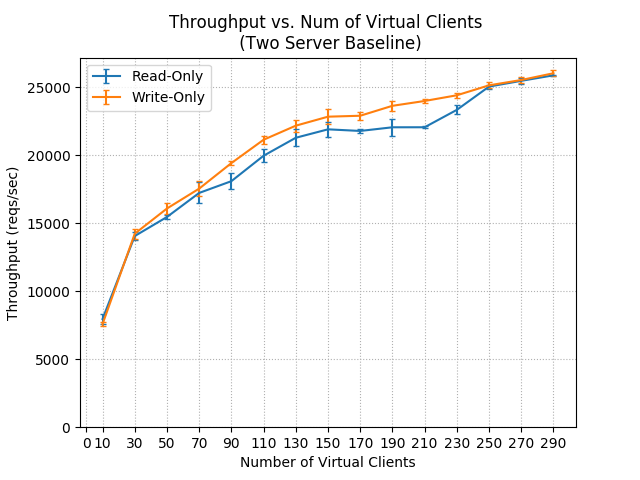
\includegraphics[scale=0.525]{images/2b_two_mc_tps.png}
		\caption{Average Throughput for baseline without middleware, \\ two memcached servers}
		\label{tps_2_mc_baseline}
	\end{minipage}\hfill
	\begin{minipage}{0.5\textwidth}
		\centering
		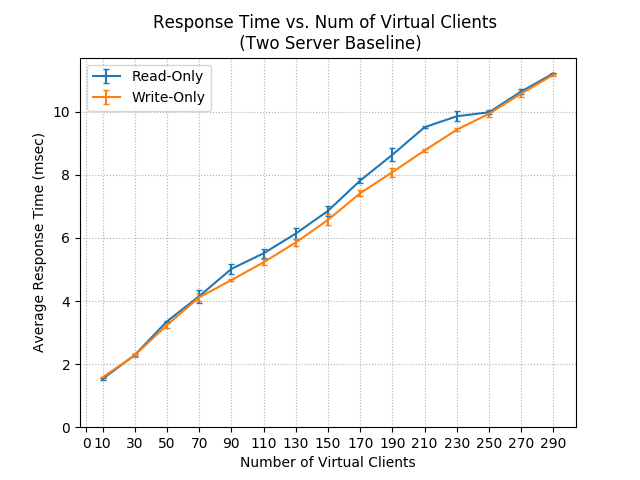
\includegraphics[scale=0.525]{images/2b_two_mc_rt.png}
		\caption{Average Response Time for baseline without middleware, \\ two memcached servers}
	\end{minipage}
\end{figure}

\subsubsection{Explanation}

% \instructions{ Describe how this experiment compares to the previous section. Which results are the same and which ones differ? Explain what further conclusions can be drawn from the experiment.}

From the throughputs plotted in Figure. \ref{tps_2_mc_baseline}, we can see that the throughput is starting to flatten out at the range of 270 to 290 clients.Thus we can say that the memcached server is undersaturated whenever the number of clients is less than 290. Saturation starts from above this number of virtual clients.

When we introduce an extra memcached server, we see that the plots of both throughput and response times for the two kinds of load we use are almost similar (within error bounds, of course). This is in contrast to the one server experiments where clearly saw that the SETs took longer than the GETs. This hints at the fact that memcached could be the bottleneck when there was only one MC server. This hypothesis will be verified in the summary.

Apart from this, two interesting observations can be made. We notice that around 190 to 210 virtual clients, the throughput of reads is noticeably lower than that of writes. The latencies are similarly higher. Above and below this range, the two work loads mirror each other in both throughput and latency. Even after repeating the experiment for multiple times, at different times, this pattern was observed. Thus, this can be attributed to issues with how the virtual machines are networked and noise in the cloud.

The second observation is that for a given number of virtual clients on the X axis, the throughput for two memcached servers is actually lower than for the same number of virtual clients in the one server case. This can be attributed to two factors. 

The first is CPU load. In the single server experiment, there were three load generating machines sending requests to a single memcached instance, in the two server server experiment, it is one load generating VM for two memcached instances. Thus, the CPU in this VM has to perform more tasks for the same number of virtual clients. For instance, in read-only experiments with 135 virtual clients per thread, \texttt{dstat} reports an average CPU utilization of 5\% for the one server experiments and 40\% for the two server experiments (these logs are at \texttt{logs/2a\_one\_server\_base\_line\_log} and \texttt{logs/2b\_two\_server\_base\_line\_log}). In other words, the CPU has to perform more work for the same number of virtual clients.

The second is the network latency. Taking a look at the average ping times at \texttt{logs/\\2a\_one\_server\_base\_line\_log/ping*}) and \texttt{logs/2b\_two\_server\_base\_line\_log/ping*}), we see that some connections can have average ping latencies that are double or triple that of other connections. These factor into reducing the number of requests that are processed as each request takes longer to reach the memcached server. These differences in latencies remained consistent even after allocating and deallocating the VMs multiple times. Nevertheless, the trends observed in the throughput is informative.


\subsection{Summary}

The experiments done in previous sections can be summarized as below. Here, VC refers to the total number of virtual clients, summed across all memtier threads and load generating VMs.

\begin{center}
	{Maximum throughput of different VMs.}
	\begin{tabular}{|l|p{2cm}|p{2cm}|p{4cm}|}
		\hline                        & Read-only workload & Write-only workload & Configuration gives max. throughput \\ 
		\hline One memcached server   & 30698 & 27894 & 210 VC (both cases)  \\ 
		\hline One load generating VM & 25881 & 26035 & 290 VC (both cases)  \\ 
		\hline 
	\end{tabular}
\end{center}

We have already discussed why the observed throughputs are different in the two situations. With all the information collected from the above two sections, we can now discuss the bottleneck in this setup. 

In the section with one memcached server, we saw that the SETs took longer than the GETs and in the section with two memcached servers, we see that both SETs and GETs take about similar times. Additionally, for a given number of virtual clients, GETs in both one server and two server setups took about similar amount of time. Thus, adding an extra server helped in reducing the response time for SETs but did not reduce the response times for the GETs.

This shows that memcached server is the bottleneck in single server experiments. To be more specific, the incoming network buffers in the memcached instances are the bottleneck. This can be explained by the fact that GET requests are smaller than SETs and as a result, occupy smaller space in the incoming network buffers at the memcached server. By doubling the number of servers, we are halving the load on each of the servers and effectively doubling the buffer size between the two servers. This means that more SETs could be read into the buffer and processed. This is a plausible reason for the trends we observe in the two previous sections.

It is also interesting to note why we don't see such buffer size issues with GETs because a response to a GET is larger than response to SETs. This could be explained by the fact that we run memcached in a single threaded mode (with flag \texttt{-t 1}) and so will process requests one by one, consequently, not putting too much load on the outgoing network buffers when compared to the load on the incoming network buffer due to multiple clients sending requests at the same time.

As already discussed in the previous section, the memtier clients form the bottleneck for the two server experiments.

Some of the takeaway messages are that we should keep an eye out for the difference in latencies across different connections in our setup and consider how they may affect our observations. Another message is to consider the lower level information like kernel buffer sizes because the memcached servers run on A1 VMs which have only 1 CPU core and are the least powerful of all the VMs we use, thus the limits to their capabilities could be a result of them being under-powered 

% \instructions{Write at least two paragraphs about how both results relate. Describe what is the bottleneck of this setup is. If the maximum throughput for both experiments is the same, explain why. If it is not the case, explain why not. Write down key take-away messages about the behaviour of the memtier clients and the memcached servers.}

\section{Baseline with Middleware} % TODO

%\instructions{ In this set of experiments, you will have to use 1 load generator VM and 1 memcached server, measuring how the throughput of the system changes when increasing the number of clients. Scaling virtual clients inside memtier has to be done as explained in the previous sections. Plot both throughput and response time as measured on the middleware.}


\subsection{One Middleware}

%\instructions{Connect one load generator machine (one instance of memtier with CT=2) to a single middleware and use 1 memcached server. Run a read-only and a write-only workload with increasing number of clients (between 2 and 64) and measure response time \emph{both at the client and at the middleware}, and plot the throughput and response time measured in the middleware. \\
%Repeat this experiment for different number of worker threads inside the middleware: 8, 16, 32, 64.}

\subsubsection{Commands}
The following are commands used to start memtier and middleware instances \\
{\scriptsize
		memtier instance: \\
			For Write-Only Loads: \texttt{memtier\_benchmark -s <MW\_IP> -p 6969 -P memcache\_text -t 2 -c <NUM\_VC\_PER\_THREAD> \\ --ratio 1:0 -d 1024 --test-time 80 --json-out-file <LOG\_FILE>} \\
			For Read-Only Loads:  \texttt{memtier\_benchmark -s <MW\_IP> -p 6969 -P memcache\_text -t 2 -c <NUM\_VC\_PER\_THREAD> \\ --ratio 0:1 -d 1024 --test-time 80 --json-out-file <LOG\_FILE>} \\
		memcached instance: \texttt{memcached -t 1 -p 6969} \\
		middleware instance: \texttt{java -jar /home/sgokula/middleware-sgokula.jar -l <MW\_IP> -p 6969 -t <NUM\_WORKER\_THREAD> -s false -m <MC\_IP>:6969}} \\
Here, \texttt{<MW\_IP>} refers to the private IP of the middleware VM (A A4 Class VM). The log file naming convention can be found in the \texttt{logs/README} file of the repository.
\subsubsection{Experimental Configuration}
\begin{center}
	\scriptsize{
		Experimental Configuration for One Middleware baseline Experiments
		\begin{tabular}{|l|c|}
			\hline Number of servers                & 1                          \\ 
			\hline Number of client machines        & 1                          \\ 
			\hline Instances of memtier per machine & 1                          \\ 
			\hline Threads per memtier instance     & 2                          \\
			\hline Virtual clients per thread       & [2, 4, 8, 16, 32, 64, 128] \\ 
			\hline Workload                         & Write-only and Read-only   \\
			\hline Multi-Get behaviour               & N/A                        \\
			\hline Multi-Get size                   & N/A                        \\
			\hline Number of middlewares            & 1                          \\
			\hline Worker threads per middleware    & [8, 16, 32, 64]            \\
			\hline Repetitions                      & 3 (1 minute steady state)  \\ 
			\hline 
		\end{tabular}
	} 
\end{center}

\subsubsection{Plots}

\begin{figure}[H]
	\captionsetup{font=scriptsize,labelfont=scriptsize,justification=centering}
	\centering
	\begin{minipage}{0.5\textwidth}
		\centering
		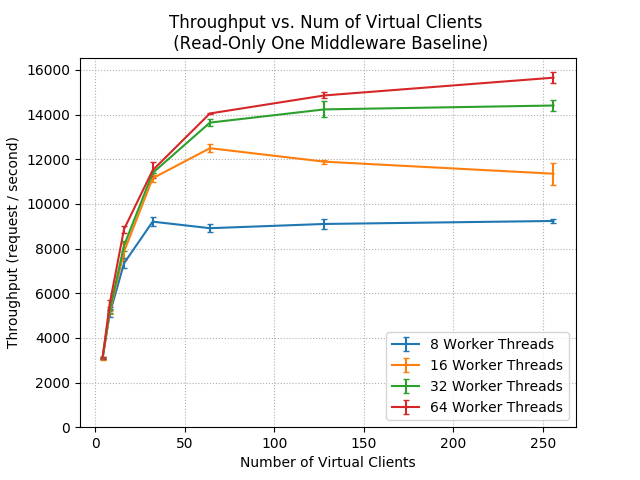
\includegraphics[scale=0.525]{images/3a_one-mw_r-o_tps.png}
		\caption{Baseline with One Middleware, Average Throughput (Read-Only Loads)}
	\end{minipage}\hfill
	\begin{minipage}{0.5\textwidth}
		\centering
		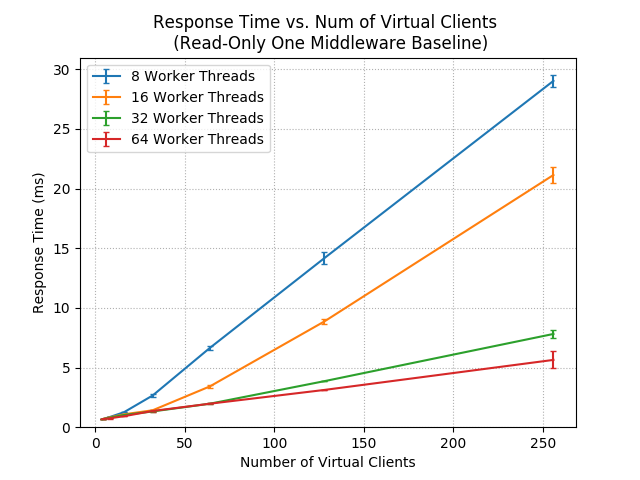
\includegraphics[scale=0.525]{images/3a_one-mw_r-o_rt.png}
		\caption{{Baseline with One Middleware, Average Response Time (Read-Only Loads)}}
	\end{minipage}
\end{figure}

\begin{figure}[H]
	\captionsetup{font=scriptsize,labelfont=scriptsize,justification=centering}
	\centering
	\begin{minipage}{0.5\textwidth}
		\centering
		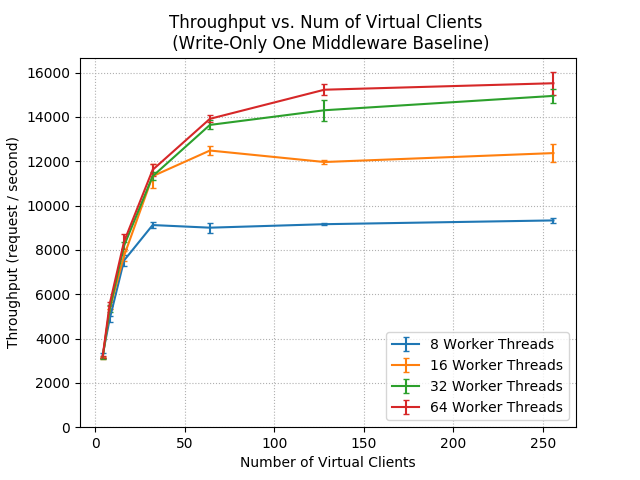
\includegraphics[scale=0.525]{images/3a_one-mw_w-o_tps.png}
		\caption{{Baseline with One Middleware, Average Throughput (Write-Only Loads)}}
	\end{minipage}\hfill
	\begin{minipage}{0.5\textwidth}
		\centering
		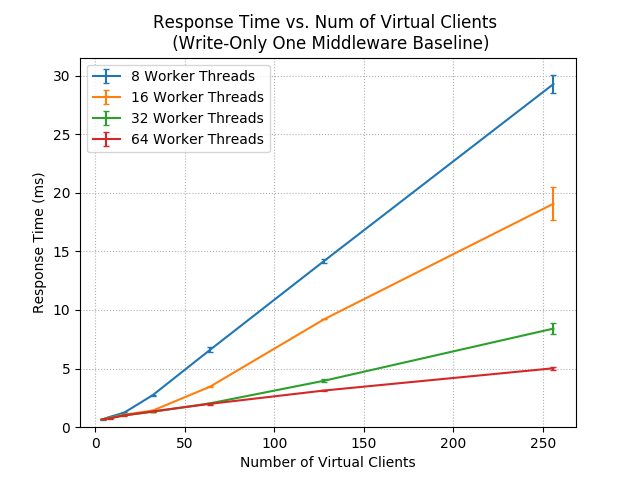
\includegraphics[scale=0.525]{images/3a_one-mw_w-o_rt.png}
		\caption{{Baseline with One Middleware, Average Response Time (Write-Only Loads)}}
	\end{minipage}
\end{figure}

\subsubsection{Explanation}

%\instructions{Provide a detailed analysis of the results (e.g., bottleneck analysis, component utilizations, average queue lengths, system saturation). Add any additional figures and experiments that help you illustrate your point and support your claims.}
From figures above, we can see that the trends and numbers for GETs and SETs are similar. This holds even though the middleware has to replicate SETs to all the memcached servers because there is only memcached server in our setup. Thus, we are seeing the same behaviour between the two request types just like we saw in the previous section.

From figures 8 and 10, we see that the middleware reaches saturation at 32, 64, 128 and 256 virtual clients when the there are 8, 16, 32 and 64 worker threads respectively. For 8 and 16 worker threads, we also observe the oversaturation phase when there are more than 32 and 64 clients as we observe the throughput dropping for these situations.

To understand why the throughput doesn't increase as we further increase the number of clients in each of the above saturation cases, let's take a look at the queuing time (time spent by a request in the queue) for each of these cases.

\begin{figure}[H]
	\captionsetup{font=scriptsize,labelfont=scriptsize,justification=centering}
	\centering
	\begin{minipage}{0.5\textwidth}
		\centering
		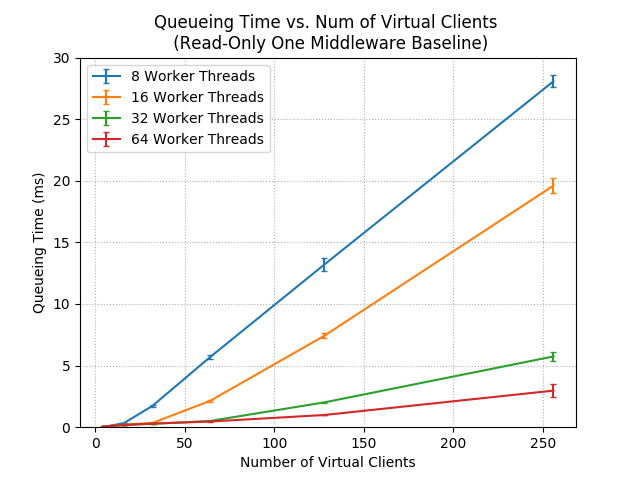
\includegraphics[scale=0.525]{images/3a_one-mw_r-o_wt.png}
		\caption{{Baseline with One Middleware, Average Queuing Time (Read-Only Loads)}}
	\end{minipage}\hfill
	\begin{minipage}{0.5\textwidth}
		\centering
		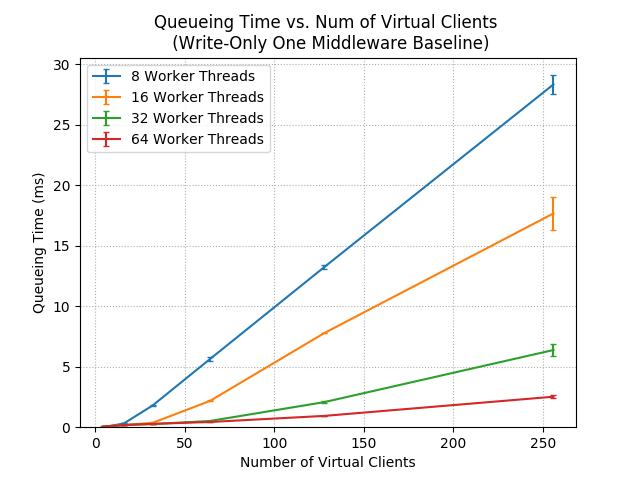
\includegraphics[scale=0.525]{images/3a_one-mw_w-o_wt.png}
		\caption{{Baseline with One Middleware, Average Queuing Time (Write-Only Loads)}}
	\end{minipage}
\end{figure}

We see that beyond the saturation point we described above, the plots for response time and queuing time are almost similar. This shows that beyond the saturation point, the requests spend significant amount of time in the queue waiting to be processed than actually being serviced. The middleware can process only \texttt{|NUM\_WORKER\_THREAD|} at any given point so any additional request will have to wait for one of the worker threads to become free before it can be processed. These waiting times are marginal when compared to the processing time whenever \texttt{|NUM\_VIRTUAL\_CLIENTS|< 4*|NUM\_WORKER\_THREAD|} (empirically from the plots) and increase rapidly when more clients are further added, as seen in the plots above.
Thus, as we increase clients further, the throughput does not increase because the worker threads are already busy most of the time. The requests, instead spend more time in the queue increasing the response time.

From these arguments, we can conclude that of memtier, middleware and memcached servers, the middleware is the bottleneck because we have seen throughputs in the 20000 - 30000 ranges without the middleware in the previous section. Inside the middleware, the worker threads are the most utilized (as they are busy most of the time) and as a result are the bottleneck in these experiments.

\subsection{Two Middlewares}

%\instructions{Connect one load generator machine (two instances of memtier with CT=1) to two middlewares and use 1 memcached server. Run a read-only and a write-only workload with increasing number of clients (between 2 and 64) and measure response time \emph{both at the client and at the middleware}, and plot the throughput and response time as measured in the middleware.\\
%Repeat this experiment for different number of worker threads inside the middleware: 8, 16, 32, 64.\\
%If in your experiment the middleware is not the bottleneck, repeat the experiment that reaches the highest throughput but using two load generator VMs (each with 2x memtier CT=1) instead of one. Otherwise, explain how you know that the middlewares are the limiting factor in terms of throughput.}

\subsubsection{Commands}
The following are the commands used to start the memtier, middleware and memcached instances \\
{\scriptsize memcached instance: \texttt{memcached -t 1 -p 6969} \\
middleware instances: \\
	\texttt{java -jar /home/sgokula/middleware-sgokula.jar -l <MW\_IP\_1> -p 6969 -t <NUM\_WORKER\_THREAD> -s false -m <MC\_IP>:6969} \\
	\texttt{java -jar /home/sgokula/middleware-sgokula.jar -l <MW\_IP\_2> -p 6969 -t <NUM\_WORKER\_THREAD> -s false -m <MC\_IP>:6969} \\
memtier instance: \\
	For Write-Only Loads: \\
		\texttt{memtier\_benchmark -s <MW\_IP\_1> -p 6969 -P memcache\_text -t 1 -c <NUM\_VC\_PER\_THREAD> --ratio 1:0 -d 1024 \\ --test-time 80 --json-out-file <LOG\_FILE>} \\
		\texttt{memtier\_benchmark -s <MW\_IP\_2> -p 6969 -P memcache\_text -t 1 -c <NUM\_VC\_PER\_THREAD> --ratio 1:0 -d 1024 \\ --test-time 80 --json-out-file <LOG\_FILE>} \\
	For Read-Only Loads: \\
		\texttt{memtier\_benchmark -s <MW\_IP\_1> -p 6969 -P memcache\_text -t 1 -c <NUM\_VC\_PER\_THREAD> --ratio 0:1 -d 1024 \\ --test-time 80 --json-out-file <LOG\_FILE>} \\
		\texttt{memtier\_benchmark -s <MW\_IP\_2> -p 6969 -P memcache\_text -t 1 -c <NUM\_VC\_PER\_THREAD> --ratio 0:1 -d 1024 \\ --test-time 80 --json-out-file <LOG\_FILE>} \\
		} \\


\subsubsection{Experimental Configuration}
\begin{center}
	\scriptsize{
		Experimental Configuration for Two Middleware baseline Experiments
		\begin{tabular}{|l|c|}
			\hline Number of servers                & 1                          \\ 
			\hline Number of client machines        & 1                          \\ 
			\hline Instances of memtier per machine & 2                          \\ 
			\hline Threads per memtier instance     & 1                          \\
			\hline Virtual clients per thread       & [2, 4, 8, 16, 32, 64, 128] \\ 
			\hline Workload                         & Write-only and Read-only   \\
			\hline Multi-Get behaviour               & N/A                        \\
			\hline Multi-Get size                   & N/A                        \\
			\hline Number of middlewares            & 2                          \\
			\hline Worker threads per middleware    & [8, 16, 32, 64]            \\
			\hline Repetitions                      & 3 (1 minute steady state)  \\ 
			\hline 
		\end{tabular}
	} 
\end{center}

\subsubsection{Plots}
% \paragraph{Read-Only}

\begin{figure}[H]
	\captionsetup{font=scriptsize,labelfont=scriptsize,justification=centering}
	\centering
	\begin{minipage}{0.5\textwidth}
		\centering
		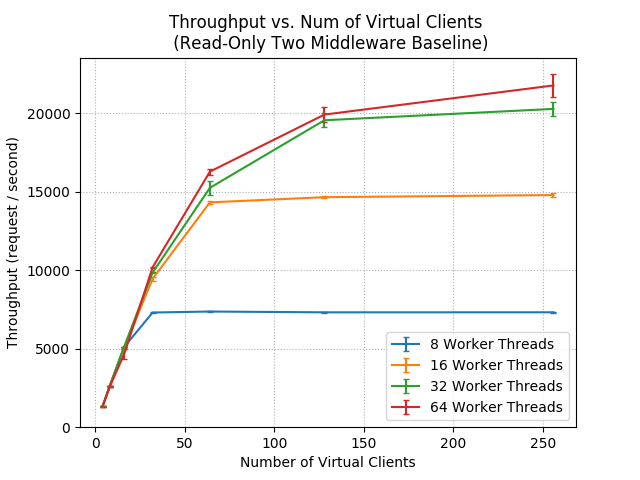
\includegraphics[scale=0.525]{images/3b_two-mw_r-o_tps.png}
		\caption{Baseline with Two Middlewares, Average Throughput (Read-Only Loads)}
	\end{minipage}\hfill
	\begin{minipage}{0.5\textwidth}
		\centering
		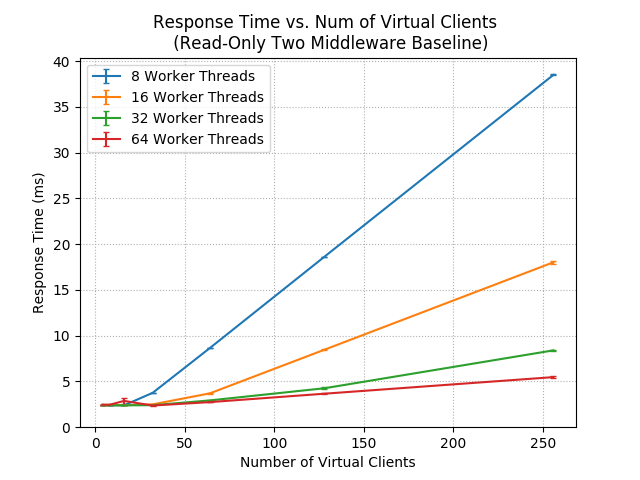
\includegraphics[scale=0.525]{images/3b_two-mw_r-o_rt.png}
		\caption{Baseline with Two Middlewares, Average Response Time (Read-Only Loads)}
	\end{minipage}
\end{figure}

\begin{figure}[H]
	\captionsetup{font=scriptsize,labelfont=scriptsize,justification=centering}
	\centering
	\begin{minipage}{0.5\textwidth}
		\centering
		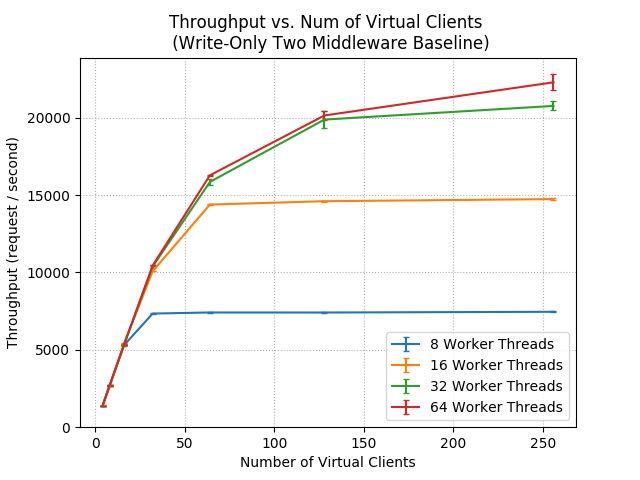
\includegraphics[scale=0.525]{images/3b_two-mw_w-o_tps.png}
		\caption{Baseline with Two Middlewares, Average Throughput (Write-Only Loads)}
	\end{minipage}\hfill
	\begin{minipage}{0.5\textwidth}
		\centering
		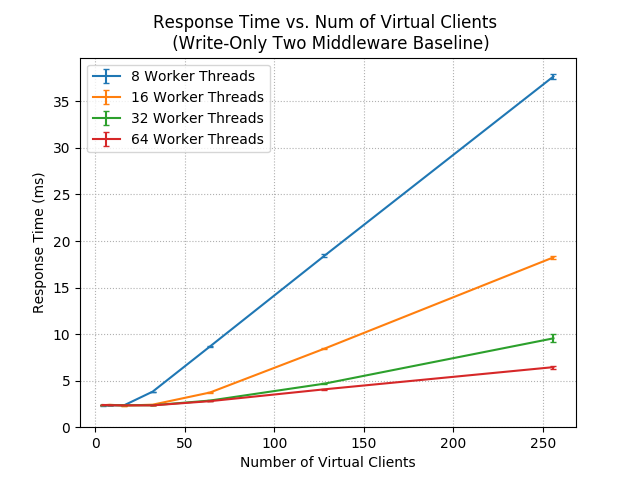
\includegraphics[scale=0.525]{images/3b_two-mw_w-o_rt.png}
		\caption{Baseline with Two Middlewares, Average Response Time (Write-Only Loads)}
	\end{minipage}
\end{figure}

\subsubsection{Explanation}

%\instructions{Provide a detailed analysis of the results (e.g., bottleneck analysis, component utilizations, average queue lengths, system saturation). Add any additional figures and experiments that help you illustrate your point and support your claims.}

Just like the section with one middleware, we see that the trends for SETs and GETs mirror each other. This shows that, even in the two middleware setup, the middleware is able to handle both types of requests in a similar way. Interestingly, the middleware saturates at the same number of virtual clients as we see in the one middleware case i.e., the middleware saturates at 32, 64, 128 and 256 clients when there are 8, 16, 32 and 64 worker threads per middleware respectively. However, the peak throughput achieved in each of these cases is higher than observed with only one middleware. The subtlety here is that 8, 16, 32 and 64 are the worker threads per middleware and in fact there are 16, 32, 64 and 128 in these cases when combining both the middlewares. Thus, we see that the individual middlewares behave just like a single middleware behaved in the previous section. Combining the two middlewares simply increased the throughput while maintaining the trends observed before. Thus, we can use the same arguments as before about the bottlenecks and utilizations of the different components of the middlewares.

The queuing time plots are shown below.
\begin{figure}[H]
	\captionsetup{font=scriptsize,labelfont=scriptsize,justification=centering}
	\centering
	\begin{minipage}{0.5\textwidth}
		\centering
		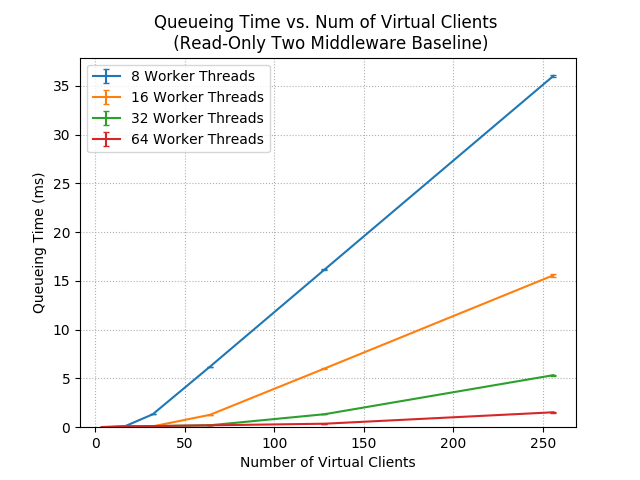
\includegraphics[scale=0.525]{images/3b_two-mw_r-o_wt.png}
		\caption{{Baseline with Two Middleware, Average Queuing Time (Read-Only Loads)}}
	\end{minipage}\hfill
	\begin{minipage}{0.5\textwidth}
		\centering
		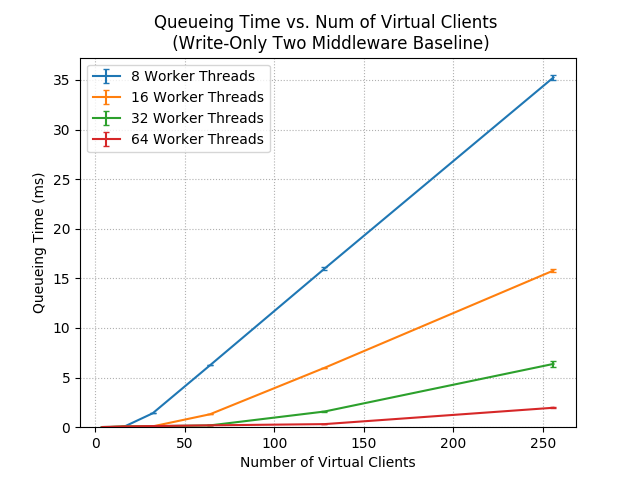
\includegraphics[scale=0.525]{images/3b_two-mw_w-o_wt.png}
		\caption{{Baseline with Two Middleware, Average Queuing Time (Write-Only Loads)}}
	\end{minipage}
\end{figure}

To ensure that the load generating VM is not the bottleneck, we can check the \texttt{dstat} logs, found at \texttt{logs/3b\_two\_mw\_base\_line/mt\_log}. We see that the CPU utilization is barely 5\% at the saturation points, this shows that that the load generating VM is not being stressed at the saturation point. Thus, we can conclude that, like before, the middleware is the bottleneck. More specifically, the worker threads of the middleware is the bottleneck and increasing them by doubling the number of middlewares (keeping the number of threads per middleware constant) increases the throughput.

\subsection{Summary}

The experiments in the above sections can be summarized as below, these numbers are averaged across repetitions to reduce the effect of random noise in the system.
%\instructions{Based on the experiments above, fill out the following table. For both of them use the numbers from a single experiment to fill out all lines. Miss rate represents the percentage of GET requests that return no data. Time in the queue refers to the time spent in the queue between the net-thread and the worker threads.}


\begin{center}
	{Maximum throughput for one middleware.}
	\begin{tabular}{|l|p{2cm}|p{2cm}|p{2cm}|p{2cm}|}
		\hline                                & Throughput & Response time(msec) & Average time in queue(msec) & Miss rate \\ 
		\hline Reads: Measured on middleware  & 15652.98   & 5.64          & 2.97                  & 0.00      \\ 
		\hline Reads: Measured on clients     & 10112.42   & 19.3          & n/a                   & 0.00      \\ 
		\hline Writes: Measured on middleware & 15521.47   & 5.02	       & 2.52                  & n/a       \\ 
		\hline Writes: Measured on clients    &  13580.12  & 18.86         & n/a                   & n/a       \\ 
		\hline 
	\end{tabular}
\end{center}

\begin{center}
	{Maximum throughput for two middlewares.}
	\begin{tabular}{|l|p{2cm}|p{2cm}|p{2cm}|p{2cm}|}
		\hline                                & Throughput & Response time(msec) & Average time in queue(msec) & Miss rate \\ 
		\hline Reads: Measured on middleware  & 21758.16   & 5.47          & 1.53                  & 0.00      \\ 
		\hline Reads: Measured on clients     & 19037.3    & 13.48         & n/a                   & 0.00      \\ 
		\hline Writes: Measured on middleware & 22291.02   & 6.45          & 1.96                  & n/a       \\ 
		\hline Writes: Measured on clients    & 19502.47   &   13.13       & n/a                   & n/a       \\ 
		\hline 
	\end{tabular}
\end{center}

%\instructions{Based on the data provided in these tables, write at least two paragraphs summarizing your findings about the performance of the middleware in the baseline experiments.}
From the above two tables we see that the response times as measured on the clients is higher than that observed on the middleware. This is because the response time at clients involve the network latency between the clients and middleware thus adding to the value. Also, we see that the throughput observed at clients is lower than that observed in middleware. This seemingly contradictory observation does not mean that there is something odd going on. This is merely because of the fact that to compute throughput, memtier considers the entire 80 seconds we run experiments. By doing so, it includes the warm-up and cool-downs phases where there are fewer requests per second. While reporting throughput for the middleware, we remove the first 5 and last 5 seconds as warm-up and cool-down phase. This explains the observed disparity. Moreover, multiplying the throughput at client by 80 and multiplying the throughput at middleware by 70 give similar numbers as expected.

We also see that, inside the middleware, the requests spend more than 30\% of the time waiting in queue, clearly indicating that the worker threads are the bottleneck. Further, throughput for both the workloads in the two middleware setup is more than the corresponding values in one middleware setup further strengthening the claim that the middleware is the bottleneck as adding an extra middleware helped increase the throughput.


%\todo{ Use sharding to explain why there's higher response time for SETs, maybe not}
\section{Throughput for Writes} % TODO

\subsection{Full System}

%\instructions{Connect three load generating VMs to two middlewares and three memchached servers. Run a write-only experiment. You need to plot throughput and response time measured on the middleware as a function of number of clients. The measurements have to be performed for 8, 16, 32 and 64 worker threads inside each middleware.}

\subsubsection{Commands}
The following are the commands used to start the memtier, middleware and memcached instances \\
{\scriptsize
memtier instance (on each load generating VM): \\
\texttt{memtier\_benchmark -s <MW\_IP\_1> -p 6969 -P memcache\_text -t 1 -c <NUM\_VIRTUAL\_CLIENTS> -d 1024 --ratio 1:0 \\ --test-time 80 --json-out-file <LOG\_FILE>} \\
\texttt{memtier\_benchmark -s <MW\_IP\_2> -p 6969 -P memcache\_text -t 1 -c <NUM\_VIRTUAL\_CLIENTS> -d 1024 --ratio 1:0 \\ --test-time 80 --json-out-file <LOG\_FILE>} \\
memcached instances: \texttt{memcached -t 1 -p 6969} \\
middleware instances: \\
\texttt{java -jar middleware-sgokula.jar -l <MW\_IP\_1> -p 6969 -t <NUM\_MW\_THREAD> -s false \\ -m <MC\_IP\_1>:6969 <MC\_IP\_2>:6969 <MC\_IP\_3>:6969} \\
\texttt{java -jar middleware-sgokula.jar -l <MW\_IP\_2> -p 6969 -t <NUM\_MW\_THREAD> -s false \\ -m <MC\_IP\_1>:6969 <MC\_IP\_2>:6969 <MC\_IP\_3>:6969} \\
}
The naming convention for the log files are mentioned in the appendix and in the \texttt{logs/README} file in the repository.
\subsubsection{Experimental Configuration}


\begin{center}
	\scriptsize{
		Experimental Configuration for "Throughput for Writes" Experiment
		\begin{tabular}{|l|c|}
			\hline Number of servers                & 3          \\ 
			\hline Number of client machines        & 3          \\ 
			\hline Instances of memtier per machine & 2          \\ 
			\hline Threads per memtier instance     & 1          \\
			\hline Virtual clients per thread       & [1, 6, 12, 18, 24, 30, 32] \\ 
			\hline Workload                         & Write-only \\
			\hline Multi-Get behaviour               & N/A        \\
			\hline Multi-Get size                   & N/A        \\
			\hline Number of middlewares            & 2          \\
			\hline Worker threads per middleware    & [8, 16, 32, 64]           \\
			\hline Repetitions                      &  3 (1 minute steady state)\\ 
			\hline 
		\end{tabular}
	} 
\end{center}

\subsubsection{Plots}

\begin{figure}[H]
	\captionsetup{font=scriptsize,labelfont=scriptsize,justification=centering}
	\centering
	\begin{minipage}{0.5\textwidth}
		\centering
		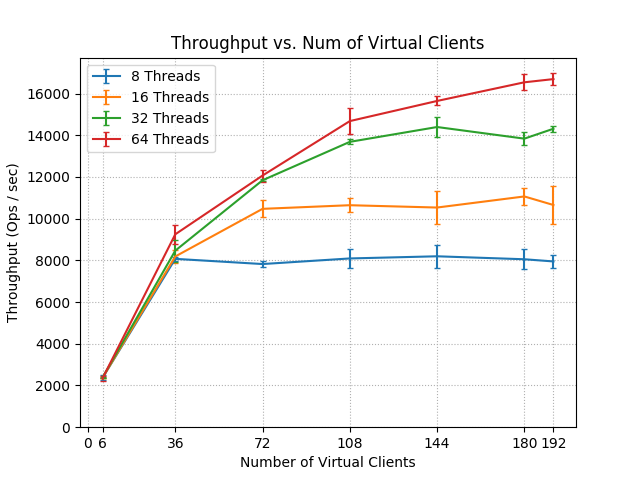
\includegraphics[scale=0.5]{images/4_set_tps_tps.png}
		\caption{Average Throughput for Sets Throughput Experiments}		
	\end{minipage}\hfill
	\begin{minipage}{0.5\textwidth}
		\centering
		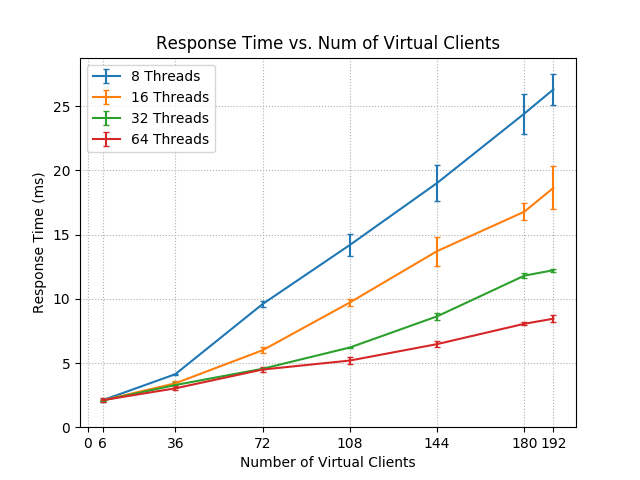
\includegraphics[scale=0.5]{images/4_set_tps_rt.png}
		\caption{Average Response Time for Sets Throughput Experiments}
	\end{minipage}
\end{figure}


\subsubsection{Explanation}

%\instructions{Provide a detailed analysis of the results (e.g., bottleneck analysis, component utilizations, average queue lengths, system saturation). Add any additional figures and experiments that help you illustrate your point and support your claims.}

From the plots above, we see the middleware getting saturated at 36, 72, 108 and 192 virtual clients when there are 8, 16, 32 and 64 worker threads per middleware respectively. We also see some signs of over-saturation and system instability to the right of these points as the throughput drops and there is higher variance in the observed throughput, indicating that the system is exhibiting erratic behaviour. We also see that the throughput at saturation increases when we increase the number of threads indicating that the middlewares do not become a bottleneck because of lack of compute or memory resources. They become a bottleneck due to a lack of parallelism brought by having a larger number of worker threads. 

To further back up our claim about the saturation point, let's look at the plots of queuing time and average queue length for these situations.

\begin{figure}[H]
	\captionsetup{font=scriptsize,labelfont=scriptsize,justification=centering}
	\centering
	\begin{minipage}{0.5\textwidth}
		\centering
		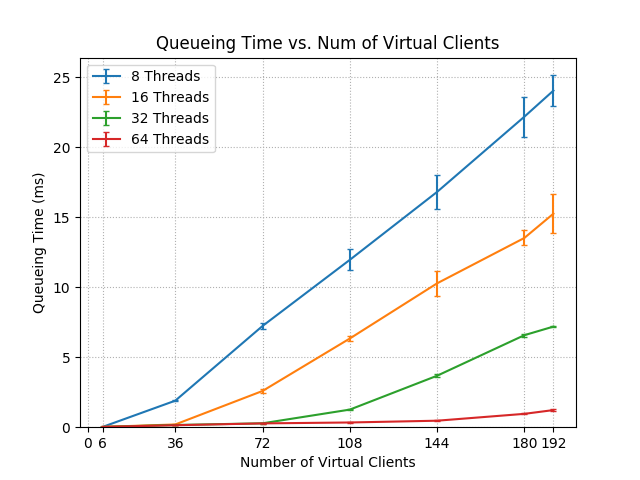
\includegraphics[scale=0.5]{images/4_set_tps_q_wt.png}
		\caption{Average Queuing Time for Sets Throughput Experiments}		
	\end{minipage}\hfill
	\begin{minipage}{0.5\textwidth}
		\centering
		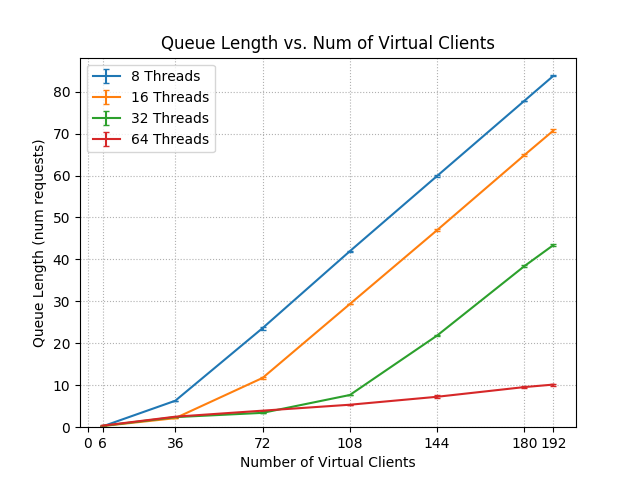
\includegraphics[scale=0.5]{images/4_set_tps_q_len.png}
		\caption{Average Queue Length for Sets Throughput Experiments}
	\end{minipage}
\end{figure}

we see that the average queue length and queuing time explode when we increase the number of cents above the saturation point. This means that as we increase clients further, the worker threads and hence the middleware itself is unable to process the request fast enough and the incoming requests are put in a queue. Since the queue gets logger and longer, the queuing get bigger and bigger as well.



\subsection{Summary}

Based on the experiments above, we can extract the following information about the maximum write throughput achieved for different setups.

\begin{center}
	{Maximum throughput for the full system}
	\begin{tabular}{|l|p{1.5cm}|p{1.5cm}|p{1.5cm}|p{1.5cm}|}
		\hline                                            & WT=8    & WT=16    & WT=32    & WT=64    \\ 
		\hline Throughput (Middleware)                    & 8072    & 10470.12 & 13682.36 & 16691.45 \\ 
		\hline Throughput (Derived from MW response time) & 8720    & 12020    & 17419.35  & 22711.42 \\ 
		\hline Throughput (Client)                        & 7062.83 & 9175.8   & 11998.7  & 14624.21 \\ 
		\hline Average time in queue                      & 1.89    & 2.58     & 1.25     & 1.22     \\ 
		\hline Average length of queue                    & 6.3     & 11.74    & 7.67     & 10.16    \\ 
		\hline Average time waiting for memcached         & 2.21    & 3.37     & 4.92     & 7.2      \\ 
		\hline Response Time at Middleware                 & 4.128   & 5.99     & 6.2      & 8.45     \\
		\hline Total Number of clients at max. TPS        & 36      & 72       & 108      & 192      \\
		\hline 
	\end{tabular}
\end{center}

%\instructions{Based on the data provided in these tables, draw conclusions on the state of your system for a variable number of worker threads.}
Here too, like in the middleware baseline experiments, the throughput measured at the clients is consistently lower than that measured on the middleware. The same reasoning used in the previous sections apply here as well. Across the columns, as we increase the number of worker threads, the middleware is able to make better use of the compute resources, increasing the throughput significantly for marginal increase in response time. This again shows that the lack of parallelism is the bottleneck.

We also see that the average time waiting for memcached increases. This is because the middleware replicates SETs across all memcached servers. As a result, as you increase the number of worker threads, the load on a single memcached server increases. Since these are under-powered, A1 VMs, they become the bottleneck as you increase the number of worker threads further. 

In fact, the start of this trend is already visible at T=64 worker threads, where requests spend a large amount of time waiting for the memcached server's response. In these cases, further increasing the number of worker threads will not help. 

In summary, at lower number of worker threads, the number of worker threads in the middleware is the bottleneck. As you increase the number of worker threads beyond 64, the memcached servers become the bottleneck due to the middleware replicating SETs across all the servers, overloading them.

It is also interesting to note that the interactive law consistently predicts higher throughput than what we measure at the middleware. This is because while computing the throughput from the interactive law, we assume that the think time (Z) is zero to simplify our calculations. This is not the case when it comes to the middleware because there are delays introduced by the network connections between the MT instances and the MW instances. Thus, this explains why predict higher throughput. The thinking time (Z) can be approximated as the difference between the response time measured at the clients and at the middleware. We shall incorporate this into our analysis and get a better estimate for throughput in the section on network of queues.



\section{Gets and Multi-gets} % TODO

%\instructions{For this set of experiments you will use three load generating machines, two middlewares and three memcached servers. Each memtier instance should have 2 virtual clients in total and the number of middleware worker threads is 64, or the one that provides the highest throughput in your system (whichever number of threads is smaller). \\
%For multi-GET workloads, memtier will generate a mixture of SETs, GETs, and multi-GETs. Memtier only allows to specify the maximum number of keys in a multi-GET request. Therefore, be aware that requests can also contain fewer keys than the provided value. It is recommended to record the average size of the multi-GETs. You will have to measure response time on the client as a function of multi-get size, with and without sharding on the middlewares.}

\subsection{Sharded Case}

%\instructions{Run multi-gets with 1, 3, 6 and 9 keys (memtier configuration) with sharding enabled (multi-gets are broken up into smaller multi-gets and spread across servers). Plot average response time as measured on the client, as well as the 25th, 50th, 75th, 90th and 99th percentiles.}

\subsubsection{Commands}
The following are the commands used to start the memtier, middleware and memcached instances
{\scriptsize
memtier instance (for each VM) \\ 
\texttt{memtier\_benchmark -s <MC\_IP\_1> -p 6969 -P memcache\_text -t 1 -c 2 --ratio 1:<MULTI\_GET\_KEY> --multi-key-get=<MULTI\_GET\_KEY> --test-time 80 --key-maximum 10000 -d 1024 --json-out-file <LOG\_FILE>} \\
\texttt{memtier\_benchmark -s <MC\_IP\_2> -p 6969 -P memcache\_text -t 1 -c 2 --ratio 1:<MULTI\_GET\_KEY> --multi-key-get=<MULTI\_GET\_KEY> --test-time 80 --key-maximum 10000 -d 1024 --json-out-file <LOG\_FILE>} \\
memcached instance: \texttt{memcached -t 1 -p 6969} \\
middleware instances: \\
	\texttt{java -jar middleware-sgokula.jar -l <MW\_IP\_1> -p 6969 -t <NUM\_WORKER\_THREAD> -s True \\ -m <MC\_IP\_1>:6969 <MC\_IP\_2>:6969 <MC\_IP\_3>:6969} \\
	\texttt{java -jar middleware-sgokula.jar -l <MW\_IP\_2> -p 6969 -t <NUM\_WORKER\_THREAD> -s True \\ -m <MC\_IP\_1>:6969 <MC\_IP\_2>:6969 <MC\_IP\_3>:6969} \\ 
}
Here, \texttt{<MC\_IP\_1>} and \texttt{<MC\_IP\_2>} refer to the private IPs of the two middlewares. \texttt{<MULTI\_GET\_KEY>} refers to the number of keys in a multi-GET request. This could be 1, 3, 6 or 9. \texttt{<NUM\_WORKER\_THREAD>} refers to the number of worker threads per middleware.

\subsubsection{Experimental Configuration}
\begin{center}
	\scriptsize{
		Experimental Configuration for Sharded Gets Experiments
		\begin{tabular}{|l|c|}
			\hline Number of servers                & 3                       \\ 
			\hline Number of client machines        & 3                       \\ 
			\hline Instances of memtier per machine & 2                       \\ 
			\hline Threads per memtier instance     & 1                       \\
			\hline Virtual clients per thread       & 2     		            \\ 
			\hline Workload                         & memtier-default (with \texttt{--ratio 1:Multi-GET-size}) \\
			\hline Multi-Get behaviour               & Sharded                 \\
			\hline Multi-Get size                   & [1, 3, 6, 9]                  \\
			\hline Number of middlewares            & 2                       \\
			\hline Worker threads per middleware    & max. throughput config.(64 Worker Threads) \\
			\hline Repetitions                      & 3 (1 minute steady state)\\ 
			\hline 
		\end{tabular}
	} 
\end{center}

\subsubsection{Plots}
	\begin{figure}[H]
		\captionsetup{font=scriptsize,labelfont=scriptsize,justification=centering}
		\centering
		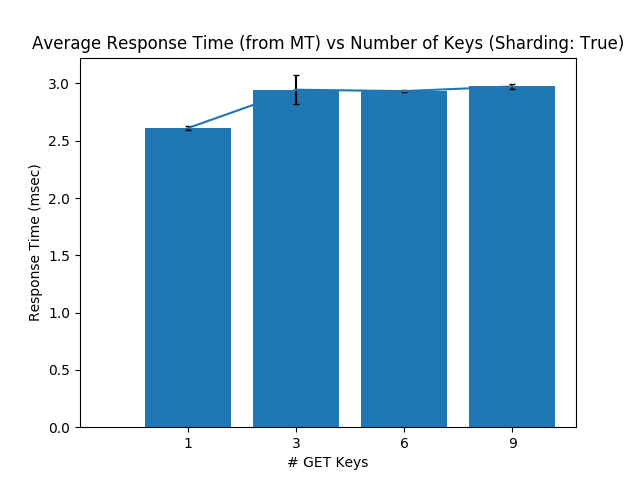
\includegraphics[scale=0.5]{images/5_shard_True_avg_r_times_mt.png}
		\caption{Average Response Time at Client (Sharded Mode)}
	\end{figure}

\begin{figure}[H]
	\captionsetup{font=scriptsize,labelfont=scriptsize,justification=centering}
	\centering
	\begin{minipage}{0.5\textwidth}
		\centering
		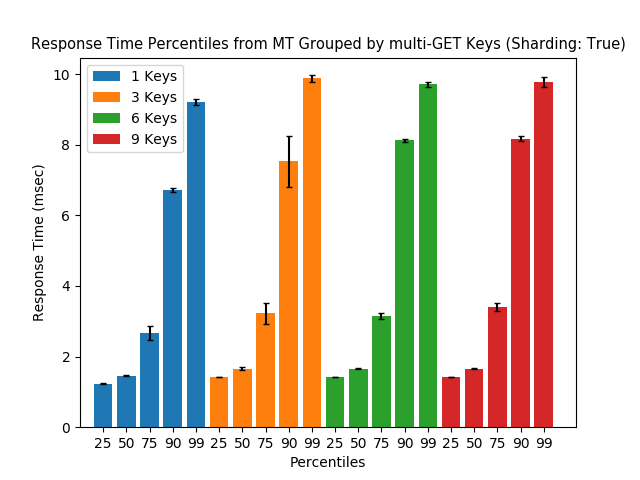
\includegraphics[scale=0.5]{images/5_shard_True_percentiles_group_by_keys_mt.png}
		\caption{Response Time at client Percentiles \\ Group by num keys (Sharded Mode)}
	\end{minipage}\hfill
	\begin{minipage}{0.5\textwidth}
		\centering
		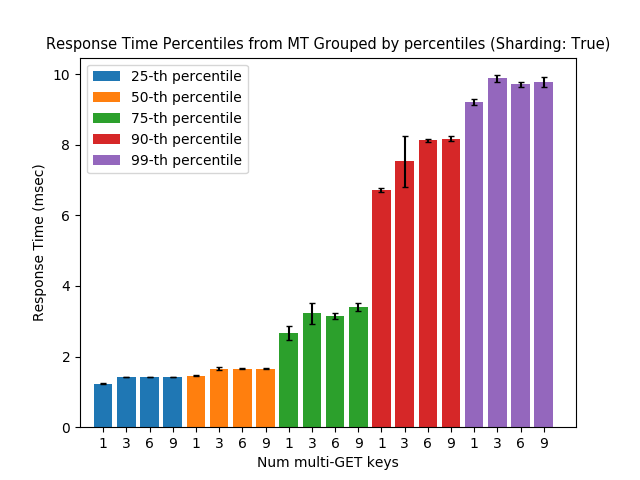
\includegraphics[scale=0.5]{images/5_shard_True_percentiles_group_by_percentile_mt.png}
		\caption{Response Time at client Percentiles \\ Group by percentile (Sharded Mode)}
	\end{minipage}
\end{figure}

\subsubsection{Explanation}

%\instructions{Provide a detailed analysis of the results (e.g., bottleneck analysis, component utilizations, average queue lengths, system saturation). Add any additional figures and experiments that help you illustrate your point and support your claims.}
In the sharded case, the middleware breaks down the multi-GET into individual keys and assigns keys to multiple smaller multi-GETs in a round robin fashion until all keys have been assigned. These are sent to the memcached servers one after the other, reading the responses only after sending all the requests. The responses are combined at the middleware and sent back to the client. Due to the \texttt{-ratio 1:<MULTI\_GET\_KEY>} flag. Our workloads consist entirely of equal number of SETs and multi-GETs with \texttt{<MULTI\_GET\_KEY>} keys. From the table above, we can see that this can take values 1, 3, 6, 9 only. When the value is 1 ,the mult-gets are treated like single GETs and are assigned to a single server in a round-robin fashion. When it is higher, each of the 3 memcached server gets a multi-GET request with exactly \texttt{<MULTI\_GET\_KEY> / 3} key. This implies that thanks to our sharding policy, each of the memcached server is equally loaded in each of our sharded experiments.

This further explains the average response time plot. The response times for 3, 6 and 9 keys are almost similar are higher than response time for 1 key. This is because of the overheads of sharding, sending to and reading from multiple servers (3x the network I/O) as well as combining the response. All these combine to give us a higher response time. Since the response time doesn't change much inbetweeen 3, 6 and 9 keys. We can conclude that in the sharded case, the actual size of data being written into the network doesn't matter as much as the number of times we write into it.

This allows us to conclude that the sharding process is the bottleneck in our middleware. More specifically, the higher number of network I/Os created by the sharding process is the limiting factor to the throughput and response time we observer in our middleware.

Additionally, we see the exact trends with percentiles as well. From figure 27, we see that even the 25, 50, 75, 90 and 99 percentiles of response time for the multi-get with 3, 6 and 9 keys are similar (and greater than that for 1 key), further providing evidence to the statement above.

Finally, from figure 26, we see that the response times at different percentiles for a given number of keys increases in an exponential fashion as we increase the percentile to 99. This suggests that the response times are exponentially distributed and might be similar to a long-tailed distribution. We see this trend across all the  different number keys we conduct experiments on.
\subsection{Non-sharded Case}

%\instructions{Run multi-gets with 1, 3, 6 and 9 keys (memtier configuration) with sharding disabled. Plot average response time as measured on the client, as well as the 25th, 50th, 75th, 90th and 99th percentiles.}


\subsubsection{Commands}
The following are the commands used to start the memtier, middleware and memcached instances

{\scriptsize
	memtier instance (for each VM) \\ 
	\texttt{memtier\_benchmark -s <MC\_IP\_1> -p 6969 -P memcache\_text -t 1 -c 2 --ratio 1:<MULTI\_GET\_KEY> --multi-key-get=<MULTI\_GET\_KEY> --test-time 80 --key-maximum 10000 -d 1024 --json-out-file <LOG\_FILE>} \\
	\texttt{memtier\_benchmark -s <MC\_IP\_2> -p 6969 -P memcache\_text -t 1 -c 2 --ratio 1:<MULTI\_GET\_KEY> --multi-key-get=<MULTI\_GET\_KEY> --test-time 80 --key-maximum 10000 -d 1024 --json-out-file <LOG\_FILE>} \\
	memcached instance: \texttt{memcached -t 1 -p 6969} \\
	middleware instances: \\
	\texttt{java -jar middleware-sgokula.jar -l <MW\_IP\_1> -p 6969 -t <NUM\_WORKER\_THREAD> -s False \\ -m <MC\_IP\_1>:6969 <MC\_IP\_2>:6969 <MC\_IP\_3>:6969} \\
	\texttt{java -jar middleware-sgokula.jar -l <MW\_IP\_2> -p 6969 -t <NUM\_WORKER\_THREAD> -s False \\ -m <MC\_IP\_1>:6969 <MC\_IP\_2>:6969 <MC\_IP\_3>:6969} \\ 
}
Here, \texttt{<MC\_IP\_1>} and \texttt{<MC\_IP\_2>} refer to the private IPs of the two middlewares. \texttt{<MULTI\_GET\_KEY>} refers to the number of keys in a multi-GET request. This could be 1, 3, 6 or 9. \texttt{<NUM\_WORKER\_THREAD>} refers to the number of worker threads per middleware.
\subsubsection{Experimental Configuration}
\begin{center}
	\scriptsize{
		Experimental Configuration for Non-Sharded Gets Experiments
		\begin{tabular}{|l|c|}
			\hline Number of servers                & 3                       \\ 
			\hline Number of client machines        & 3                       \\ 
			\hline Instances of memtier per machine & 2                       \\ 
			\hline Threads per memtier instance     & 1                       \\
			\hline Virtual clients per thread       & 2                		 \\ 
			\hline Workload                         & memtier-default (with \texttt{--ratio 1:Multi-GET-size})  \\
			\hline Multi-Get behaviour               & Non-Sharded             \\
			\hline Multi-Get size                   & [1, 3, 6, 9]                  \\
			\hline Number of middlewares            & 2                       \\
			\hline Worker threads per middleware    & max. throughput config. (64 Worker Threads) \\
			\hline Repetitions                      & 3 (1 minute steady state)               \\ 
			\hline 
		\end{tabular}
	} 
\end{center}

\subsubsection{Plots}
	
	\begin{figure}[H]
		\captionsetup{font=scriptsize,labelfont=scriptsize,justification=centering}
		\centering
		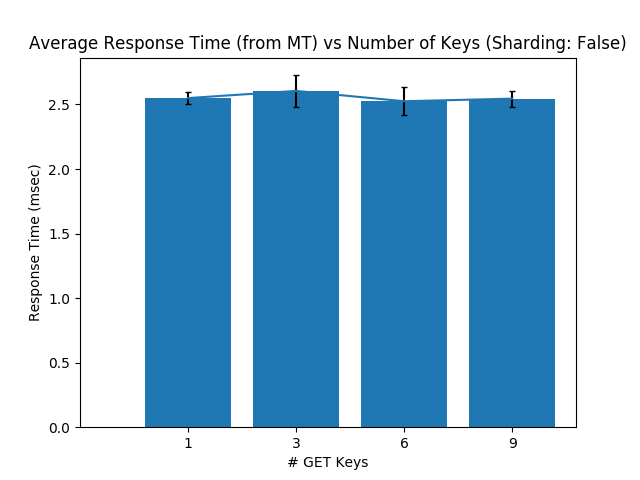
\includegraphics[scale=0.5]{images/5_shard_False_avg_r_times_mt.png}
		\caption{Average Response Time at Client (Non-Sharded Mode)}
	\end{figure}
	
	\begin{figure}[H]
		\captionsetup{font=scriptsize,labelfont=scriptsize,justification=centering}
		\centering
		\begin{minipage}{0.5\textwidth}
			\centering
			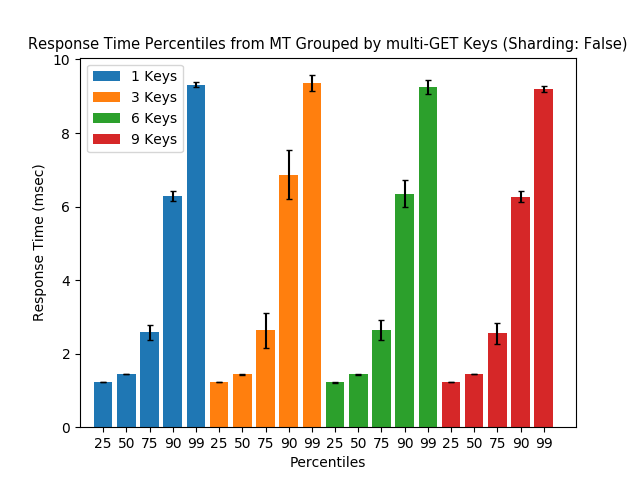
\includegraphics[scale=0.5]{images/5_shard_False_percentiles_group_by_keys_mt.png}
			\caption{Response Time at client Percentiles \\ Group by num keys (Non-Sharded Mode)}
		\end{minipage}\hfill
		\begin{minipage}{0.5\textwidth}
			\centering
			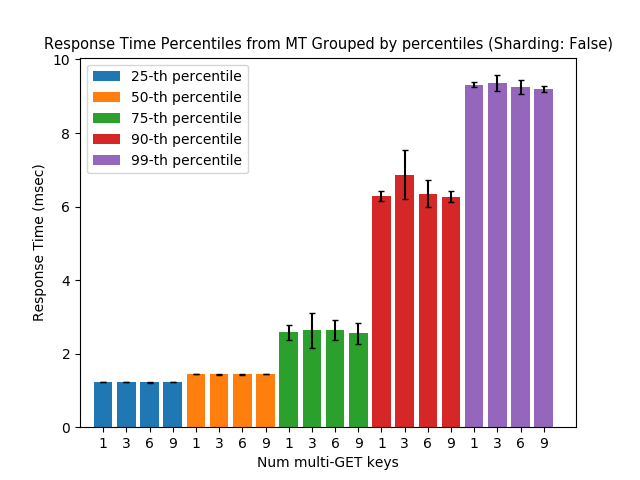
\includegraphics[scale=0.5]{images/5_shard_False_percentiles_group_by_percentile_mt.png}
			\caption{Response Time at client Percentiles \\ Group by percentile (Non-Sharded Mode)}
		\end{minipage}
	\end{figure}



\subsubsection{Explanation}

%\instructions{ Provide a detailed analysis of the results (e.g., bottleneck analysis, component utilizations, average queue lengths, system saturation). Add any additional figures and experiments that help you illustrate your point and support your claims.}
Unlike the sharded multi-gets, from figure 28, we see that the average response time is similar across all the number of keys we test on. This further provides evidence to the argument that the number of network I/O is more important than the amount of data sent during a single network I/O operation. This trend is visible in Figure 30, response time percentiles, grouped by percentiles as well. 
The rest of the argument is the same as the one from the sharded case.

We further see that the response times are lower when compared to the sharded case. This can be attributed to the absence of computations to shard the multi-GET request and join the responses from multiple servers, i.e., the response time is lower because we don't have the overheads of sharding or joining the responses.


\subsection{Histogram}

%\instructions{ For the case with 6 keys inside the multi-get, display four histograms representing the sharded and non-sharded response time distribution, both as measured on the client, and inside the middleware. Choose the bucket size in the same way for all four, and such that there are at least 10 buckets on each of the graphs.}
We choose bin sizes of 0.1 milliseconds and as many bins as to include as many of the requests in the plot as possible. Note that all of the following plots are for the case when there are 6 keys in our mulit-GET requests and we plot only the GETs at the middleware and memtier. The discussions about the histogram are included in the summary section.

%\paragraph{Sharded Mode}
\begin{figure}[H]
	\captionsetup{font=scriptsize,labelfont=scriptsize,justification=centering}
	\centering
	\begin{minipage}{0.5\textwidth}
		\centering
		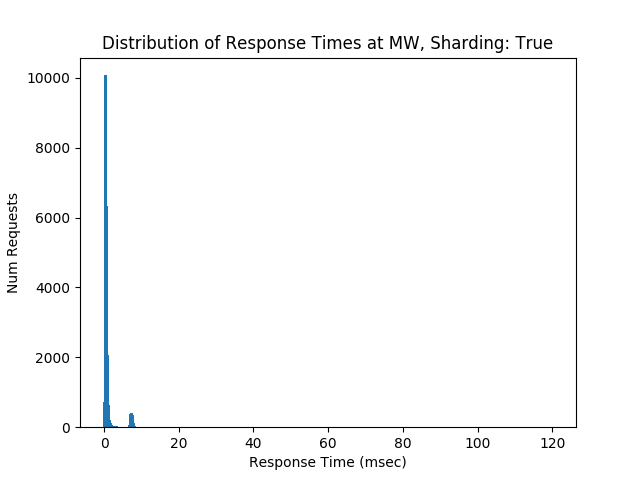
\includegraphics[scale=0.525]{images/5_mw_hist_shard_True.png}
		\caption{Response Times at Middleware, Sharding: True}
	\end{minipage}\hfill
	\begin{minipage}{0.5\textwidth}
		\centering
		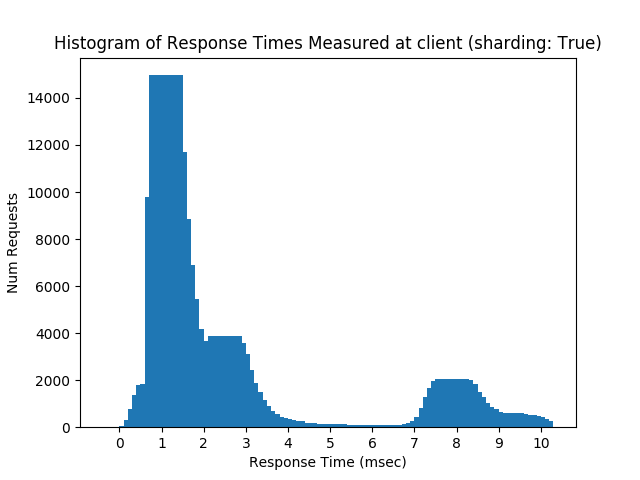
\includegraphics[scale=0.525]{images/5_mt_hist_shard_True.png}
		\caption{Response Times at Client, Sharding: True}
	\end{minipage}
\end{figure}


\begin{figure}[H]
	\captionsetup{font=scriptsize,labelfont=scriptsize,justification=centering}
	\centering
	\begin{minipage}{0.5\textwidth}
		\centering
		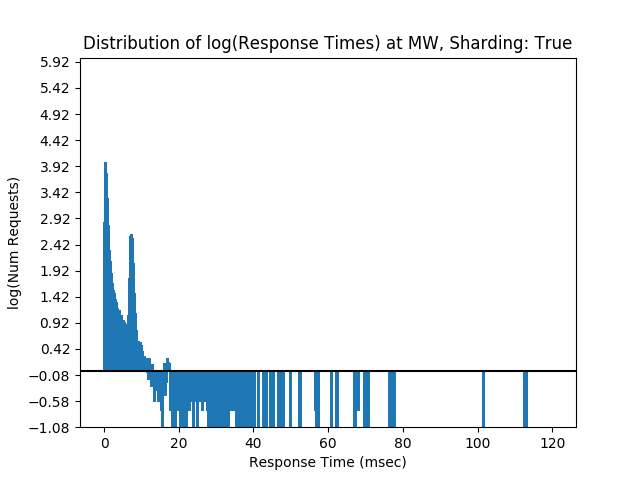
\includegraphics[scale=0.525]{images/5_mw_log_hist_shard_True.png}
		\caption{log(Response Times) at Middleware, Sharding: True}
	\end{minipage}\hfill
	\begin{minipage}{0.5\textwidth}
		\centering
		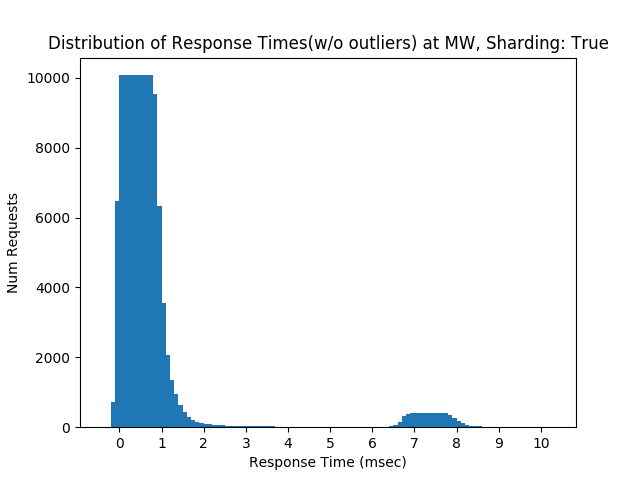
\includegraphics[scale=0.525]{images/5_mw_hist_no-outlier_shard_True.png}
		\caption{Response Times at Middleware w/o Outliers, Sharding: True}
	\end{minipage}
\end{figure}

%\paragraph{Non-Sharded Mode}
\begin{figure}[H]
	\captionsetup{font=scriptsize,labelfont=scriptsize,justification=centering}
	\centering
	\begin{minipage}{0.5\textwidth}
		\centering
		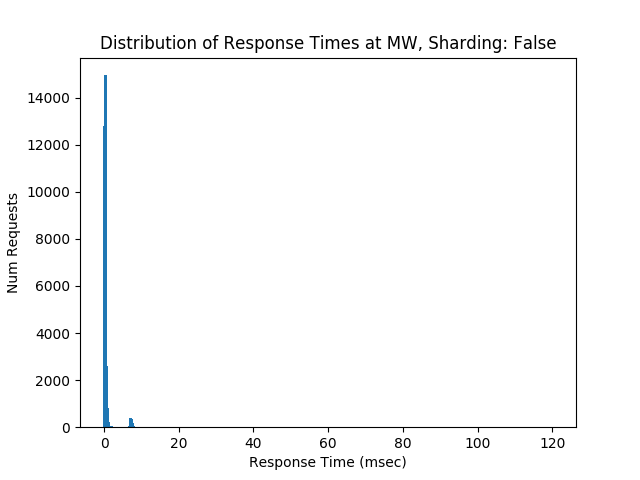
\includegraphics[scale=0.525]{images/5_mw_hist_shard_False.png}
		\caption{Response Times at Middleware, Sharding: False}
	\end{minipage}\hfill
	\begin{minipage}{0.5\textwidth}
		\centering
		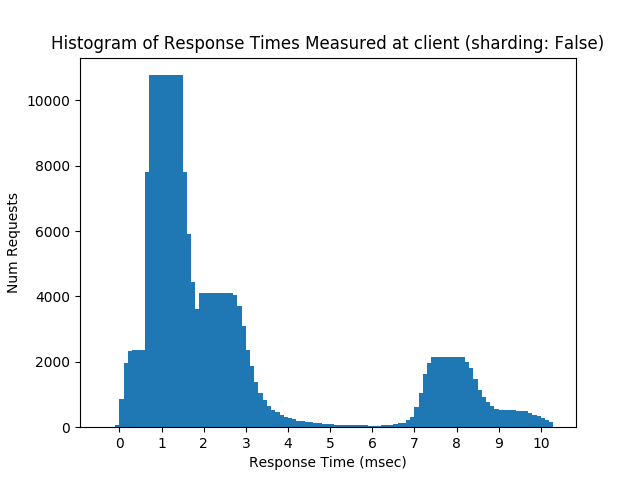
\includegraphics[scale=0.525]{images/5_mt_hist_shard_False.png}
		\caption{Response Times at Client, Sharding: False}
	\end{minipage}
\end{figure}


\begin{figure}[H]
	\captionsetup{font=scriptsize,labelfont=scriptsize,justification=centering}
	\centering
	\begin{minipage}{0.5\textwidth}
		\centering
		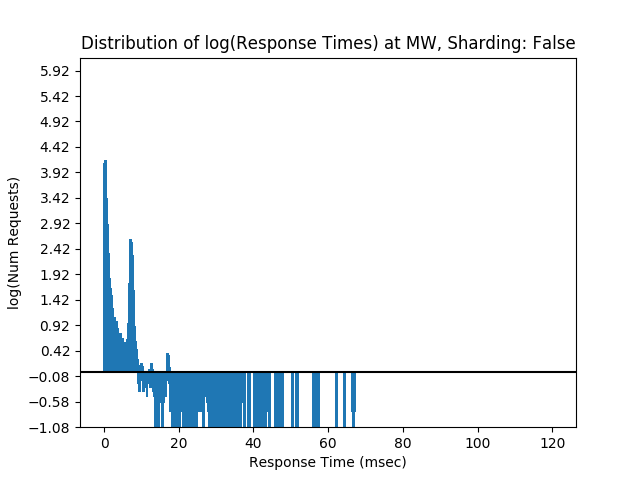
\includegraphics[scale=0.525]{images/5_mw_log_hist_shard_False.png}
		\caption{log(Response Times) at Middleware, Sharding: False}
	\end{minipage}\hfill
	\begin{minipage}{0.5\textwidth}
		\centering
		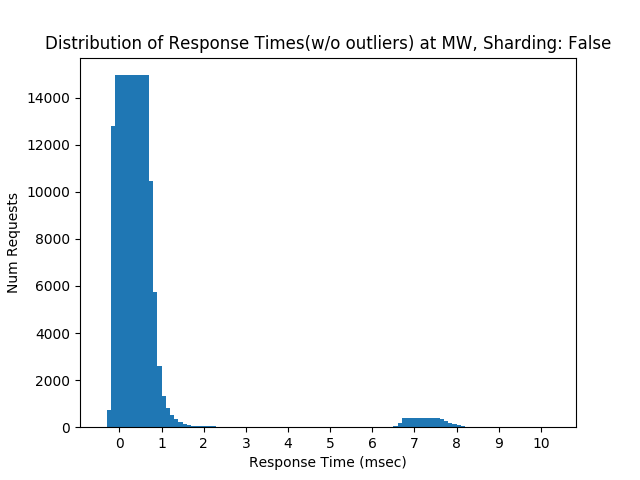
\includegraphics[scale=0.525]{images/5_mw_hist_no-outlier_shard_False.png}
		\caption{Response Times at Middleware w/o Outliers, Sharding: False}
	\end{minipage}
\end{figure}


\subsection{Summary}

%\instructions{Provide a detailed comparison of the sharded and non-shareded modes. For which multi-GET size is sharding the preferred option? Provide a detailed analysis of your system. Add any additional figures and experiments that help you illustrate your point and support your claims.}

From the histograms in figures 31 and 35, we notice that they are extremely sharp and concentrated at a very small area. To check if there are any outlier, we plot the histograms in a log scale in figures 33 and 37 and these reveal that there are indeed small numbers of requests ( < 10 ) in the higher bins. These could be due to many reasons like sudden increase in network latencies, garbage collector running, stragglers in the servers which are taking a long time to process .etc. These outliers explain the exponential behaviour in the percentile plots we saw before. We then remove the outliers (response time > 10 ms) and plot the histograms in figures 34 and 38. 
To plot the histogram from middleware, we consider only those requests that have < 10 ms response time. In all the cases, this covers 98+ \% of the requests.

Comparing these plots, we observe that the middleware has more or less the same response time across all the requests in both sharded and non-sharded case (except for a small bump near 7 to 8 msec). We see higher spread in the response times measured at the client indicating that there is a larger variance in the network latencies between the clients and the middleware than inbetween the middleware and the servers. We see these trends for both sharded and non-sharded cases.

Finally, while comparing between the sharded and non-sharded case, we see that the response times of the sharded case is higher because of the sharding and multiple network I/O overheads. For multi-GET sizes > 6, the size of the requests starts to play a more important role and thus sharding will start to be preferred than the non-sharded case when we have more than 6 keys in our multi-GETs.


\section{2K Analysis}

\subsection{Experiment Overview}

\subsubsection{Variables}
For our 2K analysis, we observe the changes in throughput and response time of the middleware while we vary the following parameters.  All the GET requests have only one key and there are 3 client machines (with 64 total virtual clients per client VM).

\begin{table}[h]
	\centering
	\caption{Factors used in the 2k-r analysis}
	\label{my-label}
	\begin{tabular}{|l|l|l|l|}
		\hline
		\textbf{Symbol} & \textbf{Factor} & \textbf{Level -1} & \textbf{Level +1} \\ \hline
		A      & Memcached servers             & 2        & 3        \\ \hline
		B      & Middlewares                   & 1        & 2        \\ \hline
		C      & Worker Threads per Middleware & 8        & 32       \\ \hline
	\end{tabular}
\end{table}

We repeat the experiment for write-only, read-only, and a 50-50-read-write workloads as well. 
We use the memtier logs from the clients to get the numbers in the subsequent sections.  The logs are at \texttt{logs/6\textunderscore 2k\textunderscore exp\textunderscore log} directory in the project's repository. The experimental configuration is as shown below

\subsubsection{Experimental Configuration}
\begin{center}
	\scriptsize{
		\begin{tabular}{|l|c|}
			\hline Number of servers                & 2 and 3                                     \\ 
			\hline Number of client machines        & 3                                           \\ 
			\hline Instances of memtier per machine & 2                                           \\ 
			\hline Threads per memtier instance     & 1                                           \\
			\hline Virtual clients per thread       & 32                                     \\ 
			\hline Workload                         & Write-only, Read-only, and 50-50-read-write \\
			\hline Multi-Get behaviour               & N/A                                         \\
			\hline Multi-Get size                   & N/A                                         \\
			\hline Number of middlewares            & 1 and 2                                     \\
			\hline Worker threads per middleware    & 8 and 32                                    \\
			\hline Repetitions                      & 3 (1 minute steady state)                   \\ 
			\hline 
		\end{tabular}
	} 
\end{center}
 The exact commands used depends on the exact configuration in question, for example, one vs two memcached instances. Thus, it is suggested to take a look at the commands from \texttt{scripts/1\_exp\_runners/5\_run\_2k.py} file.

\subsection{Write-Only Loads}
In this section, we perform a 2k-r experiment on the system when the work-load is write-only (i.e., consists only of \texttt{SET}s). 
The next two subsections display the tables from the analysis and a discussion follows afterwards.

\subsubsection{Throughput}
\begin{table}[H]
	\caption{Average Throughput for each configuration}
	\centering
	\begin{tabular}{|r|r|r|r|r|r|r|r|r|}
		\hline
		\multicolumn{1}{|l|}{I} & \multicolumn{1}{l|}{A} & \multicolumn{1}{l|}{B} & \multicolumn{1}{l|}{C} & \multicolumn{1}{l|}{AB} & \multicolumn{1}{l|}{AC} & \multicolumn{1}{l|}{BC} & \multicolumn{1}{l|}{ABC} & \multicolumn{1}{l|}{Mean Throughput} \\ \hline
		1 & -1 & -1 & -1 & 1 & 1 & 1 & -1 & 6110.47 \\ \hline
		1 & -1 & -1 & 1 & 1 & -1 & -1 & 1 & 10818.73 \\ \hline
		1 & -1 & 1 & -1 & -1 & 1 & -1 & 1 & 9275.35 \\ \hline
		1 & -1 & 1 & 1 & -1 & -1 & 1 & -1 & 17781.02 \\ \hline
		1 & 1 & -1 & -1 & -1 & -1 & 1 & 1 & 3142.77 \\ \hline
		1 & 1 & -1 & 1 & -1 & 1 & -1 & -1 & 6355.51 \\ \hline
		1 & 1 & 1 & -1 & 1 & -1 & -1 & -1 & 6609.54 \\ \hline
		1 & 1 & 1 & 1 & 1 & 1 & 1 & 1 & 12858.60 \\ \hline
	\end{tabular}
	\label{}
\end{table}

\begin{table}[H]
	\caption{Observed Throughput and errors across repetitions}
	\centering
	\begin{tabular}{|r|r|r|r|r|r|r|r|r|r|r|r|r|r|}
		\hline
		\multicolumn{1}{|l|}{I} & \multicolumn{1}{l|}{A} & \multicolumn{1}{l|}{B} & \multicolumn{1}{l|}{C} & \multicolumn{1}{l|}{AB} & \multicolumn{1}{l|}{AC} & \multicolumn{1}{l|}{BC} & \multicolumn{1}{l|}{ABC} & \multicolumn{1}{l|}{Rep\_1} & \multicolumn{1}{l|}{Rep\_2} & \multicolumn{1}{l|}{Rep\_3} & \multicolumn{1}{l|}{ERR\_1} & \multicolumn{1}{l|}{ERR\_2} & \multicolumn{1}{l|}{ERR\_3} \\ \hline
		1 & -1 & -1 & -1 & 1 & 1 & 1 & -1 & 6583.99 & 5872.06 & 5875.35 & 473.52 & -238.41 & -235.12 \\ \hline
		1 & -1 & -1 & 1 & 1 & -1 & -1 & 1 & 10784.87 & 10559.31 & 11112 & -33.86 & -259.42 & 293.27 \\ \hline
		1 & -1 & 1 & -1 & -1 & 1 & -1 & 1 & 9237.88 & 9269.57 & 9318.59 & -37.47 & -5.78 & 43.24 \\ \hline
		1 & -1 & 1 & 1 & -1 & -1 & 1 & -1 & 18600.28 & 17272.73 & 17470.06 & 819.26 & -508.29 & -310.96 \\ \hline
		1 & 1 & -1 & -1 & -1 & -1 & 1 & 1 & 3115.38 & 3198.37 & 3114.57 & -27.39 & 55.60 & -28.20 \\ \hline
		1 & 1 & -1 & 1 & -1 & 1 & -1 & -1 & 6247.53 & 6427.93 & 6391.08 & -107.98 & 72.42 & 35.57 \\ \hline
		1 & 1 & 1 & -1 & 1 & -1 & -1 & -1 & 6461.39 & 6646.43 & 6720.81 & -148.15 & 36.89 & 111.27 \\ \hline
		1 & 1 & 1 & 1 & 1 & 1 & 1 & 1 & 12841.69 & 13124.02 & 12610.09 & -16.91 & 265.42 & -248.51 \\ \hline
	\end{tabular}
	\label{}
\end{table}


\begin{table}[H]
	\begin{minipage}{.5\linewidth}
	\caption{Table of q values}
	\centering
	\begin{tabular}{|l|r|}
		\hline
		& \multicolumn{1}{l|}{Mean} \\ \hline
		q0 & 9119.00 \\ \hline
		qA & -1877.39 \\ \hline
		qB & 2512.13 \\ \hline
		qC & 2834.47 \\ \hline
		qAB & -19.66 \\ \hline
		qAC & -469.02 \\ \hline
		qBC & 854.22 \\ \hline
		qABC & -95.14 \\ \hline
	\end{tabular}
	\end{minipage}%
	\begin{minipage}{.5\linewidth}
	\caption{Sum of Squares \& Variation Contributions}
	\centering
	\begin{tabular}{|l|r|r|}
		\hline
		Component & \multicolumn{1}{l|}{Sum of Squares} & \multicolumn{1}{l|}{Contribution} \\ \hline
		SSY & 2449347512.38 & \multicolumn{1}{l|}{} \\ \hline
		SS0 & 1995747499.24 & 439.98 \\ \hline
		SST & 453600013.14 & 100.00 \\ \hline
		SSA & 84590387.28 & 18.65 \\ \hline
		SSB & 151459030.80 & \textbf{33.39} \\ \hline
		SSC & 192820830.83 & \textbf{42.51} \\ \hline
		SSAB & 9281.09 & 0.00 \\ \hline
		SSAC & 5279457.97 & 1.16 \\ \hline
		SSBC & 17512466.73 & 3.86 \\ \hline
		SSABC & 217227.45 & 0.05 \\ \hline
		SSE & 1711330.99 & 0.38 \\ \hline
	\end{tabular}
	\end{minipage} 
\end{table}

%\pagebreak
\subsubsection{Latency}

\begin{table}[!htbp]
	\caption{Average Latency(ms) for each configuration}
	\centering
	\begin{tabular}{|r|r|r|r|r|r|r|r|r|}
		\hline
		\multicolumn{1}{|l|}{I} & \multicolumn{1}{|l|}{A} & \multicolumn{1}{l|}{B} & \multicolumn{1}{l|}{C} & \multicolumn{1}{l|}{AB} & \multicolumn{1}{l|}{AC} & \multicolumn{1}{l|}{BC} & \multicolumn{1}{l|}{ABC} & \multicolumn{1}{l|}{Mean Latency} \\ \hline
		1 & -1 & -1 & -1 & 1 & 1 & 1 & -1 & 31.55 \\ \hline
		1 & -1 & -1 & 1 & 1 & -1 & -1 & 1 & 17.69 \\ \hline
		1 & -1 & 1 & -1 & -1 & 1 & -1 & 1 & 21.89 \\ \hline
		1 & -1 & 1 & 1 & -1 & -1 & 1 & -1 & 10.91 \\ \hline
		1 & 1 & -1 & -1 & -1 & -1 & 1 & 1 & 60.93 \\ \hline
		1 & 1 & -1 & 1 & -1 & 1 & -1 & -1 & 30.21 \\ \hline
		1 & 1 & 1 & -1 & 1 & -1 & -1 & -1 & 29.03 \\ \hline
		1 & 1 & 1 & 1 & 1 & 1 & 1 & 1 & 14.96 \\ \hline
	\end{tabular}
	\label{}
\end{table}


\begin{table}[H]
	\caption{Observed Latency(ms) and errors across repetitions}
	\begin{tabular}{|r|r|r|r|r|r|r|r|r|r|r|r|r|r|}
		\hline
		\multicolumn{1}{|l|}{I} & \multicolumn{1}{l|}{A} & \multicolumn{1}{l|}{B} & \multicolumn{1}{l|}{C} & \multicolumn{1}{l|}{AB} & \multicolumn{1}{l|}{AC} & \multicolumn{1}{l|}{BC} & \multicolumn{1}{l|}{ABC} & \multicolumn{1}{l|}{LAT\_1} & \multicolumn{1}{l|}{LAT\_2} & \multicolumn{1}{l|}{LAT\_3} & \multicolumn{1}{l|}{ERR\_1} & \multicolumn{1}{l|}{ERR\_2} & \multicolumn{1}{l|}{ERR\_3} \\ \hline
		1 & -1 & -1 & -1 & 1 & 1 & 1 & -1 & 29.16 & 32.83 & 32.67 & -2.40 & 1.28 & 1.12 \\ \hline
		1 & -1 & -1 & 1 & 1 & -1 & -1 & 1 & 17.80 & 17.96 & 17.31 & 0.11 & 0.27 & -0.38 \\ \hline
		1 & -1 & 1 & -1 & -1 & 1 & -1 & 1 & 22.08 & 21.83 & 21.75 & 0.19 & -0.06 & -0.14 \\ \hline
		1 & -1 & 1 & 1 & -1 & -1 & 1 & -1 & 10.33 & 11.28 & 11.11 & -0.58 & 0.37 & 0.20 \\ \hline
		1 & 1 & -1 & -1 & -1 & -1 & 1 & 1 & 61.62 & 60.04 & 61.13 & 0.69 & -0.89 & 0.20 \\ \hline
		1 & 1 & -1 & 1 & -1 & 1 & -1 & -1 & 30.73 & 29.87 & 30.04 & 0.52 & -0.34 & -0.17 \\ \hline
		1 & 1 & 1 & -1 & 1 & -1 & -1 & -1 & 29.46 & 28.97 & 28.66 & 0.43 & -0.06 & -0.37 \\ \hline
		1 & 1 & 1 & 1 & 1 & 1 & 1 & 1 & 14.99 & 14.65 & 15.24 & 0.03 & -0.31 & 0.28 \\ \hline
	\end{tabular}
	\label{}
\end{table}


\begin{table}[H]
	\begin{minipage}{.5\linewidth}
	\caption{Table of q values}
	\centering
	\begin{tabular}{|l|r|}
		\hline
		& \multicolumn{1}{l|}{Mean} \\ \hline
		q0 & 27.15 \\ \hline
		qA & 6.64 \\ \hline
		qB & -7.95 \\ \hline
		qC & -8.70 \\ \hline
		qAB & -3.84 \\ \hline
		qAC & -2.49 \\ \hline
		qBC & 2.44 \\ \hline
		qABC & 1.72 \\ \hline
	\end{tabular}
	\end{minipage}%
	\begin{minipage}{.5\linewidth}
	\caption{Sum of Squares and Variation Contribution Analysis}
	\centering
	\begin{tabular}{|l|r|r|}
		\hline
		Component & \multicolumn{1}{l|}{Sum of Squares} & \multicolumn{1}{l|}{Contribution} \\ \hline
		SSY & 22806.38 & \multicolumn{1}{l|}{} \\ \hline
		SS0 & 17685.51 & 345.36 \\ \hline
		SST & 5120.87 & 100.00 \\ \hline
		SSA & 1057.09 & 20.64 \\ \hline
		SSB & 1516.86 & \textbf{29.62} \\ \hline
		SSC & 1818.47 & \textbf{35.51} \\ \hline
		SSAB & 353.54 & 6.90 \\ \hline
		SSAC & 149.15 & 2.91 \\ \hline
		SSBC & 143.03 & 2.79 \\ \hline
		SSABC & 71.06 & 1.39 \\ \hline
		SSE & 11.66 & 0.23 \\ \hline
	\end{tabular}
	\end{minipage} 
\end{table}
%\pagebreak
\subsubsection{Discussion}
In both throughput and latency, we see that the number of Middlewares and the number of workers threads in each of the middleware contributes significantly to the observed throughput and lantency. Together they explain around 70\% of the observed variations in throughput and latency. Moreover, the interaction terms like AB, AC, AB, ABC have very small contributions to the variance indicating that the factors are not correlated. 

More specifically, the number of worker threads contributes more to the variance than the number of middlewares. To understand this, let's take a look at the definitions of throughput and latency. Throughput is the average number of jobs completed per unit time. Now, to increase this term, we either need to reduce the time taken to complete one job or increase the level of parallelism so that more jobs can be processed at the same time. In our systems, the network latency dominates the time taken to complete a request (this can be seen from any of the middleware logs in any of the sections). We cannot alter the network latency by changing any of the three factors, hence we cannot significantly reduce the amount of time a single request takes. Therefore, increasing the parallelism is the only way ahead.

Now, let's take a look at response time, it is the average amount of time a request takes to complete. As we have just seen, the network latency is the biggest contributor to the response time. Since the worker threads are synchronous, they have to wait until the response from the memcached servers comes back before processing the next request. This means that the worker threads are idle most of the time and the CPU is underutilized. Adding another middleware does not increase the utilization of a single core as you are doubling the number of cores and effectively reducing the load per core (as the requests are now split across two middlewares) when you are adding another middleware. However, by increasing the number of worker threads, you are increasing the utilization of the CPU and are effectively reducing the amount of time the middleware takes to forward the request to the memcached servers.

From the above two paragraphs, it is clear that increasing the level of parallelism will be the way to higher throughput and lower service times. Parallelism in the middleware(s) can be understood by looking at the total number of worker threads. Let's take the case when there's only one middleware with 8 worker threads (Both B and C are -1). If we were to change factor B, the number of middlewares, the total number of worker threads would be 16. Instead, if we change factor C, the number of worker threads, the total number of worker threads goes up to 32. Thus, the latter has double the effect of the former option and as a result has more effect on both the latency and throughput due to the effective increase in parallelism it introduces.

%For the throughput, increasing the number of worker threads per MW has slightly more effect than increasing the number of middlewares. To understand this, let's take a look at the definition of throughput. It is the average number of jobs completed per unit time. Now, to increase this term, we either need to reduce the time taken to complete one job or increase the parallelism so that more jobs can be processed simultaneously. In our systems, the network latency dominates the time taken to complete a request (this can be seen from any of the middleware logs in any of the sections). We cannot alter the network latency by changing any of the three factors. Therefore, increasing the parallelism is the only way ahead. Let's consider the case when Worker Threads / MW is 8. If we were to double the number of middlewares, we effectively double the total number of threads to 16. If we were to increase to number of threads instead, we quadruple the number of threads to 32.The latter option increases parallelism more than the former and thus factor C contributes more variance than factor B.


%For the latency, to understand why number of middlewares contributes more than the number of worker threads, we need to consider what exactly happens when we increase the number of middlewares from 1 to 2. 

%While doing so, we are adding 4 more CPU cores, several gigabytes of RAM as well as effectively doubling the total number of worker threads to process incoming requests all the while reducing the load on the first middleware by half (keeping the number of virtual clients fixed), effectively halving the network load per middleware instance.  These are significant changes when compared to increasing the number of threads (which in turn increases contention for CPU cycles) or increasing the number of memcached servers (which increase the time needed to replicate across all the MC servers) and reduce the time a single request takes to complete by utilizing more compute resources and reducing network traffic between a single middleware and the memcached servers. Moreover, increasing the parallelism by increasing the number of threads does not reduce the time a single request takes to complete (which factors into the latency). As a result, increasing the number of threads (factor B) contributes more variance than increasing the number of middlewares (factor C).

 
% \pagebreak
\subsection{Read-Only Loads}
In this section, we perform a 2k-r experiment on the system when the work-load is read-only (i.e., consists only of \texttt{GET}s). There are no multi-\texttt{GET}s and the memcached servers are pre-populated to avoid any GET  misses.

\subsubsection{Throughput} 
\begin{table}[H]
	\caption{Average Throughput for each configuration}
	\centering
	\begin{tabular}{|r|r|r|r|r|r|r|r|r|}
		\hline
		\multicolumn{1}{|l|}{I} & \multicolumn{1}{l|}{A} & \multicolumn{1}{l|}{B} & \multicolumn{1}{l|}{C} & \multicolumn{1}{l|}{AB} & \multicolumn{1}{l|}{AC} & \multicolumn{1}{l|}{BC} & \multicolumn{1}{l|}{ABC} & \multicolumn{1}{l|}{Mean Throughput} \\ \hline
		1 & -1 & -1 & -1 & 1 & 1 & 1 & -1 & 7141.31 \\ \hline
		1 & -1 & -1 & 1 & 1 & -1 & -1 & 1 & 12813.33 \\ \hline
		1 & -1 & 1 & -1 & -1 & 1 & -1 & 1 & 10894.01 \\ \hline
		1 & -1 & 1 & 1 & -1 & -1 & 1 & -1 & 21132.15 \\ \hline
		1 & 1 & -1 & -1 & -1 & -1 & 1 & 1 & 5537.52 \\ \hline
		1 & 1 & -1 & 1 & -1 & 1 & -1 & -1 & 11035.39 \\ \hline
		1 & 1 & 1 & -1 & 1 & -1 & -1 & -1 & 10639.02 \\ \hline
		1 & 1 & 1 & 1 & 1 & 1 & 1 & 1 & 19984.16 \\ \hline
	\end{tabular}
	\label{}
\end{table}

\begin{table}[H]
	\caption{Observed Throughput and errors across repetitions}
	\begin{tabular}{|r|r|r|r|r|r|r|r|r|r|r|r|r|r|}
		\hline
		\multicolumn{1}{|l|}{I} & \multicolumn{1}{l|}{A} & \multicolumn{1}{l|}{B} & \multicolumn{1}{l|}{C} & \multicolumn{1}{l|}{AB} & \multicolumn{1}{l|}{AC} & \multicolumn{1}{l|}{BC} & \multicolumn{1}{l|}{ABC} & \multicolumn{1}{l|}{Rep\_1} & \multicolumn{1}{l|}{Rep\_2} & \multicolumn{1}{l|}{Rep\_3} & \multicolumn{1}{l|}{ERR\_1} & \multicolumn{1}{l|}{ERR\_2} & \multicolumn{1}{l|}{ERR\_3} \\ \hline
		1 & -1 & -1 & -1 & 1 & 1 & 1 & -1 & 6894.96 & 6907.95 & 7621.01 & -246.35 & -233.36 & 479.70 \\ \hline
		1 & -1 & -1 & 1 & 1 & -1 & -1 & 1 & 12602.77 & 13113.52 & 12723.7 & -210.56 & 300.19 & -89.63 \\ \hline
		1 & -1 & 1 & -1 & -1 & 1 & -1 & 1 & 11112.42 & 10709.1 & 10860.5 & 218.41 & -184.91 & -33.51 \\ \hline
		1 & -1 & 1 & 1 & -1 & -1 & 1 & -1 & 20920.12 & 21609.2 & 20867.14 & -212.03 & 477.05 & -265.01 \\ \hline
		1 & 1 & -1 & -1 & -1 & -1 & 1 & 1 & 5270.24 & 5655.58 & 5686.73 & -267.28 & 118.06 & 149.21 \\ \hline
		1 & 1 & -1 & 1 & -1 & 1 & -1 & -1 & 10950.75 & 10764.43 & 11391 & -84.64 & -270.96 & 355.61 \\ \hline
		1 & 1 & 1 & -1 & 1 & -1 & -1 & -1 & 10710.6 & 10579.93 & 10626.53 & 71.58 & -59.09 & -12.49 \\ \hline
		1 & 1 & 1 & 1 & 1 & 1 & 1 & 1 & 20216.69 & 19582.97 & 20152.81 & 232.53 & -401.19 & 168.65 \\ \hline
	\end{tabular}
	\label{}
\end{table}


\begin{table}[H]
	\begin{minipage}{.5\linewidth}
	\caption{Table of q values}
	\centering
	\begin{tabular}{|l|r|}
		\hline
		& \multicolumn{1}{l|}{Mean} \\ \hline
		q0 & 12397.11 \\ \hline
		qA & -598.09 \\ \hline
		qB & 3265.22 \\ \hline
		qC & 3844.15 \\ \hline
		qAB & 247.34 \\ \hline
		qAC & -133.39 \\ \hline
		qBC & 1051.67 \\ \hline
		qABC & -89.86 \\ \hline
	\end{tabular}
	\end{minipage}%
	\begin{minipage}{.5\linewidth}
	\caption{Table of Sum of Squares and Variation Contribution Analysis}
	\centering
	\begin{tabular}{|l|r|r|}
		\hline
		Component & \multicolumn{1}{l|}{Sum of Squares} & \multicolumn{1}{l|}{Contribution} \\ \hline
		SSY & 4337759141.88 & \multicolumn{1}{l|}{} \\ \hline
		SS0 & 3688520320.39 & 568.13 \\ \hline
		SST & 649238821.49 & 100.00 \\ \hline
		SSA & 8585043.67 & 1.32 \\ \hline
		SSB & 255880467.30 & \textbf{39.41}\\ \hline
		SSC & 354659356.93 & \textbf{54.63} \\ \hline
		SSAB & 1468284.44 & 0.23 \\ \hline
		SSAC & 427058.76 & 0.07 \\ \hline
		SSBC & 26544382.17 & 4.09 \\ \hline
		SSABC & 193786.68 & 0.03 \\ \hline
		SSE & 1480441.54 & 0.23 \\ \hline
	\end{tabular}
	\end{minipage} 
\end{table}

\subsubsection{Latency}

\begin{table}[H]
	\caption{Average Latency(ms) for each configuration}
	\centering
	\begin{tabular}{|r|r|r|r|r|r|r|r|r|}
		\hline
		\multicolumn{1}{|l|}{I} & \multicolumn{1}{l|}{A} & \multicolumn{1}{l|}{B} & \multicolumn{1}{l|}{C} & \multicolumn{1}{l|}{AB} & \multicolumn{1}{l|}{AC} & \multicolumn{1}{l|}{BC} & \multicolumn{1}{l|}{ABC} & \multicolumn{1}{l|}{Mean Latency} \\ \hline
		1 & -1 & -1 & -1 & 1 & 1 & 1 & -1 & 26.87 \\ \hline
		1 & -1 & -1 & 1 & 1 & -1 & -1 & 1 & 14.98 \\ \hline
		1 & -1 & 1 & -1 & -1 & 1 & -1 & 1 & 19.36 \\ \hline
		1 & -1 & 1 & 1 & -1 & -1 & 1 & -1 & 9.14 \\ \hline
		1 & 1 & -1 & -1 & -1 & -1 & 1 & 1 & 34.71 \\ \hline
		1 & 1 & -1 & 1 & -1 & 1 & -1 & -1 & 17.43 \\ \hline
		1 & 1 & 1 & -1 & 1 & -1 & -1 & -1 & 18.19 \\ \hline
		1 & 1 & 1 & 1 & 1 & 1 & 1 & 1 & 9.59 \\ \hline
	\end{tabular}
	\label{}
\end{table}

\begin{table}[H]
	\caption{Observed Latency(ms) and errors across repetitions}
	\centering
	\begin{tabular}{|r|r|r|r|r|r|r|r|r|r|r|r|r|r|}
		\hline
		\multicolumn{1}{|l|}{I} & \multicolumn{1}{l|}{A} & \multicolumn{1}{l|}{B} & \multicolumn{1}{l|}{C} & \multicolumn{1}{l|}{AB} & \multicolumn{1}{l|}{AC} & \multicolumn{1}{l|}{BC} & \multicolumn{1}{l|}{ABC} & \multicolumn{1}{l|}{Rep\_1} & \multicolumn{1}{l|}{Rep\_2} & \multicolumn{1}{l|}{Rep\_3} & \multicolumn{1}{l|}{ERR\_1} & \multicolumn{1}{l|}{ERR\_2} & \multicolumn{1}{l|}{ERR\_3} \\ \hline
		1 & -1 & -1 & -1 & 1 & 1 & 1 & -1 & 27.84 & 27.79 & 24.98 & 0.97 & 0.92 & -1.89 \\ \hline
		1 & -1 & -1 & 1 & 1 & -1 & -1 & 1 & 15.23 & 14.64 & 15.08 & 0.25 & -0.35 & 0.10 \\ \hline
		1 & -1 & 1 & -1 & -1 & 1 & -1 & 1 & 19.08 & 19.61 & 19.40 & -0.28 & 0.24 & 0.04 \\ \hline
		1 & -1 & 1 & 1 & -1 & -1 & 1 & -1 & 9.27 & 8.90 & 9.24 & 0.13 & -0.24 & 0.10 \\ \hline
		1 & 1 & -1 & -1 & -1 & -1 & 1 & 1 & 36.43 & 33.94 & 33.76 & 1.72 & -0.77 & -0.95 \\ \hline
		1 & 1 & -1 & 1 & -1 & 1 & -1 & -1 & 17.53 & 17.83 & 16.92 & 0.10 & 0.41 & -0.51 \\ \hline
		1 & 1 & 1 & -1 & 1 & -1 & -1 & -1 & 18.11 & 18.29 & 18.18 & -0.09 & 0.10 & -0.01 \\ \hline
		1 & 1 & 1 & 1 & 1 & 1 & 1 & 1 & 9.51 & 9.74 & 9.52 & -0.08 & 0.15 & -0.07 \\ \hline
	\end{tabular}
	\label{}
\end{table}

\begin{table}[H]
	\begin{minipage}{.5\linewidth}
	\caption{Table of q values}
	\centering
	\begin{tabular}{|l|r|}
		\hline
		& \multicolumn{1}{l|}{Mean} \\ \hline
		q0 & 18.78 \\ \hline
		qA & 1.20 \\ \hline
		qB & -4.71 \\ \hline
		qC & -6.00 \\ \hline
		qAB & -1.38 \\ \hline
		qAC & -0.47 \\ \hline
		qBC & 1.29 \\ \hline
		qABC & 0.88 \\ \hline
	\end{tabular}
	\end{minipage}%
	\begin{minipage}{.5\linewidth}
	\caption{Table of Sum of Squares and Variation Contribution Analysis}
	\centering
	\begin{tabular}{|l|r|r|}
		\hline
		Component & \multicolumn{1}{l|}{Sum of Squares} & \multicolumn{1}{l|}{Contribution} \\ \hline
		SSY & 10019.89 & \multicolumn{1}{l|}{} \\ \hline
		SS0 & 8468.90 & 546.03 \\ \hline
		SST & 1550.98 & 100.00 \\ \hline
		SSA & 34.31 & 2.21 \\ \hline
		SSB & 532.95 & \textbf{34.36}\\ \hline
		SSC & 863.68 & \textbf{55.69} \\ \hline
		SSAB & 45.40 & 2.93 \\ \hline
		SSAC & 5.33 & 0.34 \\ \hline
		SSBC & 40.11 & 2.59 \\ \hline
		SSABC & 18.48 & 1.19 \\ \hline
		SSE & 10.71 & 0.69 \\ \hline
	\end{tabular}
	\end{minipage} 
\end{table}

\subsubsection{Discussion}
We see similar trends in the contributions to variations like seen in the write-only workload section. These can be explained with similar arguments as made before and hence will not be repeated here. An interesting observation to make is the wider gap between SSC and SSB in both throughput and latency as compared to the same quantities in the write-only work loads. In order to understand this, we need to recollect how the middleware handles SETs and Single-GETs. 

In the case of SETs, the middleware replicates the request to each of the memcached servers, for a total of $| memcached\_servers|$ network writes. For Single-GETs, the middleware simply forwards the request to just one of the memcached servers and load-balances among st the servers by using a round-robin strategy. Even though the multiple network I/Os in case of SETs are not done sequentially, it is important to remember that all worker threads are forwarding requests to all the memcached servers, increasing the memcached servers' load and consequently increasing the time the single-threaded memcached servers take to process these requests and send a response back.

Thus, the network latencies play a slighty smaller role here when compared to the write-only workload and as a result, the effective parallelism plays a more significant role. Thus, increasing the number of worker threads per middleware has more pronounced effect than increasing the number of middlewares.

\subsection{Read-Write Loads}
In this section, we perform a 2k-r experiment on the system when the work-load is read-write (50-50) (i.e., we pass \texttt{--ratio 1:1} flag to memtier to have equal number of SETs and GETs). 
\subsubsection{Throughput}

\begin{table}[H]
	\caption{Average Throughput for each configuration}
	\centering
	\begin{tabular}{|r|r|r|r|r|r|r|r|r|}
		\hline
		\multicolumn{1}{|l|}{I} & \multicolumn{1}{l|}{A} & \multicolumn{1}{l|}{B} & \multicolumn{1}{l|}{C} & \multicolumn{1}{l|}{AB} & \multicolumn{1}{l|}{AC} & \multicolumn{1}{l|}{BC} & \multicolumn{1}{l|}{ABC} & \multicolumn{1}{l|}{Mean Throughput} \\ \hline
		1 & -1 & -1 & -1 & 1 & 1 & 1 & -1 & 6356.06 \\ \hline
		1 & -1 & -1 & 1 & 1 & -1 & -1 & 1 & 11769.73 \\ \hline
		1 & -1 & 1 & -1 & -1 & 1 & -1 & 1 & 10533.18 \\ \hline
		1 & -1 & 1 & 1 & -1 & -1 & 1 & -1 & 18866.50 \\ \hline
		1 & 1 & -1 & -1 & -1 & -1 & 1 & 1 & 4007.03 \\ \hline
		1 & 1 & -1 & 1 & -1 & 1 & -1 & -1 & 7307.03 \\ \hline
		1 & 1 & 1 & -1 & 1 & -1 & -1 & -1 & 8428.42 \\ \hline
		1 & 1 & 1 & 1 & 1 & 1 & 1 & 1 & 15992.66 \\ \hline
	\end{tabular}
	\label{}
\end{table}

\begin{table}[H]
	\caption{Observed Throughput and errors across repetitions}
	\centering
	\begin{tabular}{|r|r|r|r|r|r|r|r|r|r|r|r|r|r|}
		\hline
		\multicolumn{1}{|l|}{I} & \multicolumn{1}{l|}{A} & \multicolumn{1}{l|}{B} & \multicolumn{1}{l|}{C} & \multicolumn{1}{l|}{AB} & \multicolumn{1}{l|}{AC} & \multicolumn{1}{l|}{BC} & \multicolumn{1}{l|}{ABC} & \multicolumn{1}{l|}{Rep\_1} & \multicolumn{1}{l|}{Rep\_2} & \multicolumn{1}{l|}{Rep\_3} & \multicolumn{1}{l|}{ERR\_1} & \multicolumn{1}{l|}{ERR\_2} & \multicolumn{1}{l|}{ERR\_3} \\ \hline
		1 & -1 & -1 & -1 & 1 & 1 & 1 & -1 & 6232.82 & 6180.9 & 6654.47 & -123.24 & -175.16 & 298.41 \\ \hline
		1 & -1 & -1 & 1 & 1 & -1 & -1 & 1 & 12054.08 & 11417.01 & 11838.1 & 284.35 & -352.72 & 68.37 \\ \hline
		1 & -1 & 1 & -1 & -1 & 1 & -1 & 1 & 10542.57 & 10579.65 & 10477.33 & 9.39 & 46.47 & -55.85 \\ \hline
		1 & -1 & 1 & 1 & -1 & -1 & 1 & -1 & 19360.33 & 18999.67 & 18239.5 & 493.83 & 133.17 & -627.00 \\ \hline
		1 & 1 & -1 & -1 & -1 & -1 & 1 & 1 & 3987.2 & 4015.18 & 4018.7 & -19.83 & 8.15 & 11.67 \\ \hline
		1 & 1 & -1 & 1 & -1 & 1 & -1 & -1 & 6129.36 & 7755.02 & 8036.72 & -1177.67 & 447.99 & 729.69 \\ \hline
		1 & 1 & 1 & -1 & 1 & -1 & -1 & -1 & 8354.41 & 8368.4 & 8562.45 & -74.01 & -60.02 & 134.03 \\ \hline
		1 & 1 & 1 & 1 & 1 & 1 & 1 & 1 & 16266.49 & 16348.99 & 15362.5 & 273.83 & 356.33 & -630.16 \\ \hline
	\end{tabular}
	\label{}
\end{table}

\begin{table}[H]
	\begin{minipage}{.5\linewidth}
	\caption{Table of q values}
	\centering
	\begin{tabular}{|l|r|}
		\hline
		& \multicolumn{1}{l|}{Mean} \\ \hline
		q0 & 10407.58 \\ \hline
		qA & -1473.79 \\ \hline
		qB & 3047.61 \\ \hline
		qC & 3076.40 \\ \hline
		qAB & 229.14 \\ \hline
		qAC & -360.34 \\ \hline
		qBC & 897.99 \\ \hline
		qABC & 168.07 \\ \hline
	\end{tabular}		
	\end{minipage}%
	\begin{minipage}{.5\linewidth}
	\caption{Table of Sum of Squares and Variation Contribution Analysis}
	\centering
	\begin{tabular}{|l|r|r|}
		\hline
		Component & \multicolumn{1}{l|}{Sum of Squares} & \multicolumn{1}{l|}{Contribution} \\ \hline
		SSY & 3129965586.60 & \multicolumn{1}{l|}{} \\ \hline
		SS0 & 2599623857.89 & 490.18 \\ \hline
		SST & 530341728.70 & 100.00 \\ \hline
		SSA & 52129514.52 & 9.83 \\ \hline
		SSB & 222910789.66 & \textbf{42.03} \\ \hline
		SSC & 227142240.79 & \textbf{42.83} \\ \hline
		SSAB & 1260137.10 & 0.24 \\ \hline
		SSAC & 3116314.01 & 0.59 \\ \hline
		SSBC & 19353067.41 & 3.65 \\ \hline
		SSABC & 677964.13 & 0.13 \\ \hline
		SSE & 3751701.09 & 0.71 \\ \hline
	\end{tabular}		
	\end{minipage} 
\end{table}

\subsubsection{Latency}

\begin{table}[H]
	\caption{Average Latency(ms) for each configuration}
	\centering
	\begin{tabular}{|r|r|r|r|r|r|r|r|r|}
		\hline
		\multicolumn{1}{|l|}{I} & \multicolumn{1}{l|}{A} & \multicolumn{1}{l|}{B} & \multicolumn{1}{l|}{C} & \multicolumn{1}{l|}{AB} & \multicolumn{1}{l|}{AC} & \multicolumn{1}{l|}{BC} & \multicolumn{1}{l|}{ABC} & \multicolumn{1}{l|}{Mean Latency} \\ \hline
		1 & -1 & -1 & -1 & 1 & 1 & 1 & -1 & 30.23 \\ \hline
		1 & -1 & -1 & 1 & 1 & -1 & -1 & 1 & 16.32 \\ \hline
		1 & -1 & 1 & -1 & -1 & 1 & -1 & 1 & 19.34 \\ \hline
		1 & -1 & 1 & 1 & -1 & -1 & 1 & -1 & 10.31 \\ \hline
		1 & 1 & -1 & -1 & -1 & -1 & 1 & 1 & 47.91 \\ \hline
		1 & 1 & -1 & 1 & -1 & 1 & -1 & -1 & 26.65 \\ \hline
		1 & 1 & 1 & -1 & 1 & -1 & -1 & -1 & 22.80 \\ \hline
		1 & 1 & 1 & 1 & 1 & 1 & 1 & 1 & 12.02 \\ \hline
	\end{tabular}
	\label{}
\end{table}

\begin{table}[H]
	\caption{Observed Latency(ms) and errors across repetitions}
	\centering
	\begin{tabular}{|r|r|r|r|r|r|r|r|r|r|r|r|r|r|}
		\hline
		\multicolumn{1}{|l|}{I} & \multicolumn{1}{l|}{A} & \multicolumn{1}{l|}{B} & \multicolumn{1}{l|}{C} & \multicolumn{1}{l|}{AB} & \multicolumn{1}{l|}{AC} & \multicolumn{1}{l|}{BC} & \multicolumn{1}{l|}{ABC} & \multicolumn{1}{l|}{Rep\_1} & \multicolumn{1}{l|}{Rep\_2} & \multicolumn{1}{l|}{Rep\_3} & \multicolumn{1}{l|}{ERR\_1} & \multicolumn{1}{l|}{ERR\_2} & \multicolumn{1}{l|}{ERR\_3} \\ \hline
		1 & -1 & -1 & -1 & 1 & 1 & 1 & -1 & 30.80 & 31.06 & 28.85 & 0.56 & 0.83 & -1.39 \\ \hline
		1 & -1 & -1 & 1 & 1 & -1 & -1 & 1 & 15.93 & 16.82 & 16.22 & -0.39 & 0.50 & -0.10 \\ \hline
		1 & -1 & 1 & -1 & -1 & 1 & -1 & 1 & 19.40 & 19.24 & 19.39 & 0.06 & -0.11 & 0.05 \\ \hline
		1 & -1 & 1 & 1 & -1 & -1 & 1 & -1 & 10.08 & 10.20 & 10.66 & -0.23 & -0.12 & 0.35 \\ \hline
		1 & 1 & -1 & -1 & -1 & -1 & 1 & 1 & 48.16 & 47.81 & 47.77 & 0.25 & -0.10 & -0.14 \\ \hline
		1 & 1 & -1 & 1 & -1 & 1 & -1 & -1 & 31.32 & 24.75 & 23.88 & 4.67 & -1.90 & -2.77 \\ \hline
		1 & 1 & 1 & -1 & 1 & -1 & -1 & -1 & 22.99 & 22.94 & 22.47 & 0.19 & 0.14 & -0.33 \\ \hline
		1 & 1 & 1 & 1 & 1 & 1 & 1 & 1 & 11.81 & 11.76 & 12.50 & -0.21 & -0.26 & 0.47 \\ \hline
	\end{tabular}
	\label{}
\end{table}



\begin{table}[H]
	\begin{minipage}{.5\linewidth}
	\caption{Table of q values}
	\centering
	\begin{tabular}{|l|r|}
		\hline
		& \multicolumn{1}{l|}{Mean} \\ \hline
		q0 & 23.20 \\ \hline
		qA & 4.15 \\ \hline
		qB & -7.08 \\ \hline
		qC & -6.87 \\ \hline
		qAB & -2.86 \\ \hline
		qAC & -1.14 \\ \hline
		qBC & 1.92 \\ \hline
		qABC & 0.70 \\ \hline
	\end{tabular}		
	\end{minipage}%
	\begin{minipage}{.5\linewidth}
	\caption{Table of Sum of Squares and Variation Contribution Analysis}
	\centering
	\begin{tabular}{|l|r|r|}
		\hline
		Component & \multicolumn{1}{l|}{Sum of Squares} & \multicolumn{1}{l|}{Contribution} \\ \hline
		SSY & 16030.63 & \multicolumn{1}{l|}{} \\ \hline
		SS0 & 12916.52 & 414.78 \\ \hline
		SST & 3114.10 & 100.00 \\ \hline
		SSA & 412.76 & 13.25 \\ \hline
		SSB & 1203.41 & \textbf{38.64} \\ \hline
		SSC & 1133.69 & \textbf{36.40} \\ \hline
		SSAB & 195.64 & 6.28 \\ \hline
		SSAC & 31.02 & 1.00 \\ \hline
		SSBC & 88.61 & 2.85 \\ \hline
		SSABC & 11.79 & 0.38 \\ \hline
		SSE & 37.18 & 1.19 \\ \hline
	\end{tabular}		
	\end{minipage} 
\end{table}

\subsubsection{Discussion}
In this case, just like the two discussed before, the number of worker threads and the number of middlewares contribute the most to the variation in throughput and latency. From the tables 21 and 25, it seems like the number of middlewares contributes slightly more than the number of worker threads. On a closer inspection and checking the computations in \texttt{scripts/2k\_analysis.ods}, it is clear that contributions of factor B and C are same (within error bounds)

To understand why this happens, we need to consider the fact that the read-write load has two kinds of requests, the slower SETs and the faster GETs. The potential improvements in throughput and latency of GETs is diminished because on average, the GETs are blocked by a slower SET request 50\% of the time (because there are equal number of SETs and GETs and we assume that the system at any given time has equal numbers of SETs and GETs) and have to wait for the SETs to complete first. As a result of this, we see that factors B and C end up contributing almost similar amounts to variations in throughput and latency.

\section{Queuing Model}

%\instructions{Note that for queuing models it is enough to use the experimental results from the previous sections. It is, however, possible that the numbers you need are not only the ones in the figures we asked for, but also the internal measurements that you have obtained through instrumentation of your middleware.}

\subsection{M/M/1}

%\instructions{Build queuing model based on Section 4 (write-only throughput) for each worker-thread configuration of the middleware. Use one M/M/1 queue to model your entire system. Motivate your choice of input parameters to the model. Explain for which experiments the predictions of the model match and for which they do not.}
%\todo{entire system is just MW or MW and MT?}

In this section, we will model our middleware as an M/M/1 system when there are 8, 16, 32 and 64 worker threads per middleware (or 16, 32, 64, 128 total worker threads). We will compute things like Traffic Intensity, Mean number of jobs in the system, number of jobs in the queue, response time and the waiting time. We will also compare these with the observed values from section 4 and comment on the plausible reasons for the observed deviations (if any)

The following are the maximum throughputs observed for a given number of worker threads in a single repetition. These will function as the service rate to our models. 
\begin{table}[H]
	\centering
	\caption{Maximum Observed Throughput / Service Rate}
	\begin{tabular}{|c|c|}
		\hline
		\multicolumn{1}{|c|}{Worker Threads} & \multicolumn{1}{c|}{Max TPS} \\ \hline
		8 & 8877.54   \\ \hline
		16 & 11719.44 \\ \hline
		32 & 15070.91 \\ \hline
		64 & 17069.94 \\ \hline
	\end{tabular}
\end{table}
Since we have a closed system and do not lose any requests, the average throughput in each of these cases will be the arrival rate. Once we have these two parameters, we can compute the rest using results from queuing theory as below. The exact calculations and numbers can be found in \texttt{scripts/MM1.ods} in the repository.

\begin{table}[H]
		\centering
	\caption{M/M/1 Queueing Model, $\lambda$ arrival rate, $\mu$ service rate (both jobs/sec)}
	\begin{tabular}{|c|c|}
		\hline
		\multicolumn{1}{|c|}{Parameter} & \multicolumn{1}{c|}{Formula} \\ \hline
		Traffic Intensity ($\rho$) & $\lambda/\mu$ \\ \hline
		Mean num jobs in system    & $\rho / (1-\rho)$ \\ \hline
		Mean num jobs in queue     & $ \rho^{2}/(1 - \rho)$ \\ \hline
		Mean response time         & $ (1/\mu)/(1 - \rho)$ \\ \hline
		Mean waiting time          & $\rho \frac{1/\mu}{(1 - \rho)}$ \\ \hline
	\end{tabular}
	\label{}
\end{table}
 
\subsubsection{WT 8}
For the under-saturation region, let's take Num VC = 6 and for the saturation region, Num VC = 36. These have average throughputs of 2368.2 and 8072 respectively.

\begin{table}[H]
	\centering
	\caption{M/M/1 model for WT 8, undersaturation (VC = 6)}
		\begin{tabular}{|l|r|r|r|}
		\hline
		\multicolumn{1}{|c|}{Statistics} & \multicolumn{1}{c|}{Model} & \multicolumn{1}{c|}{Measured} & \multicolumn{1}{c|}{difference} \\ \hline
		Arrival rate & \multicolumn{ 2}{c|}{2368.2000} & \multicolumn{1}{l|}{} \\ \hline
		Service rate & \multicolumn{ 2}{c|}{8877.5429} & \multicolumn{1}{l|}{} \\ \hline
		Traffic intensity (System utilization) & \multicolumn{ 2}{c|}{0.2668} & \multicolumn{1}{l|}{} \\ \hline
		Probability of zero jobs in system & \multicolumn{ 2}{c|}{0.7332} & \multicolumn{1}{l|}{} \\ \hline
		Mean number of jobs in system & 0.3638 & 16.1898 & 15.8260 \\ \hline
		Mean number of jobs in queue & 0.0971 & 0.1898 & 0.0927 \\ \hline
		Variance of number of jobs in queue & 0.1583 & 0.0009 & 0.1573 \\ \hline
		Mean response time & 0.0002 & 2.0974 & 2.0973 \\ \hline
		Variance of response time & 0.0000000 & 0.0170 & 0.0170 \\ \hline
		Mean waiting time & 0.00004 & 0.0181 & 0.0181 \\ \hline
		Variance of waiting time & 0.00 & 0.0000 & 0.0000 \\ \hline
	\end{tabular}
	\label{}

\end{table}

\begin{table}[H]
	\centering
	\caption{M/M/1 model for WT 8, saturation (VC = 36)}
	\begin{tabular}{|l|r|l|r|}
		\hline
		\multicolumn{1}{|c|}{Statistics} & \multicolumn{1}{c|}{Model} & \multicolumn{1}{c|}{Measured} & \multicolumn{1}{c|}{difference} \\ \hline
		Arrival rate & \multicolumn{ 2}{c|}{8072.0000} & \multicolumn{1}{l|}{} \\ \hline
		Service rate & \multicolumn{ 2}{c|}{8877.5429} & \multicolumn{1}{l|}{} \\ \hline
		Traffic intensity (System utilization) & \multicolumn{ 2}{c|}{0.9093} & \multicolumn{1}{l|}{} \\ \hline
		Probability of zero jobs in system & \multicolumn{ 2}{c|}{0.0907} & \multicolumn{1}{l|}{} \\ \hline
		Mean number of jobs in system & 10.0206 &  & 10.0206 \\ \hline
		Variance of number of jobs in system & 110.4324 &  & 110.4324 \\ \hline
		Mean number of jobs in queue & 9.1113 & \multicolumn{1}{r|}{6.3080} & 2.8033 \\ \hline
		Variance of number of jobs in queue & 108.6964 & \multicolumn{1}{r|}{0.0001} & 108.6963 \\ \hline
		Mean response time & 0.0012 & \multicolumn{1}{r|}{4.1283} & 4.1271 \\ \hline
		Variance of response time & 0.0000015 & \multicolumn{1}{r|}{0.0021} & 0.0021 \\ \hline
		Mean waiting time & 0.00113 & \multicolumn{1}{r|}{1.8952} & 1.8941 \\ \hline
		Variance of waiting time & 0.00 & \multicolumn{1}{r|}{0.0004} & 0.0004 \\ \hline
	\end{tabular}
	\label{}
\end{table}


\subsubsection{WT 16}
For the under-saturation region, let's take Num VC = 36 and for the saturation region, Num VC = 72. These have average throughputs of 8186 and 10470.12 respectively.

\begin{table}[H]
	\centering
	\caption{M/M/1 model for WT 16, undersaturation (VC = 36)}
	\begin{tabular}{|l|r|r|r|}
		\hline
		\multicolumn{1}{|c|}{Statistics} & \multicolumn{1}{c|}{Model} & \multicolumn{1}{c|}{Measured} & \multicolumn{1}{c|}{difference} \\ \hline
		Arrival rate & \multicolumn{ 2}{c|}{8186.0000} & \multicolumn{1}{l|}{} \\ \hline
		Service rate & \multicolumn{ 2}{c|}{11719.4429} & \multicolumn{1}{l|}{} \\ \hline
		Traffic intensity (System utilization) & \multicolumn{ 2}{c|}{0.6985} & \multicolumn{1}{l|}{} \\ \hline
		Probability of zero jobs in system & \multicolumn{ 2}{c|}{0.3015} & \multicolumn{1}{l|}{} \\ \hline
		Mean number of jobs in system & 2.3167 & 34.1553 & 31.8386 \\ \hline
		Mean number of jobs in queue & 1.6182 & 2.1553 & 0.5371 \\ \hline
		Variance of number of jobs in queue & 6.4975 & 0.0022 & 6.4953 \\ \hline
		Mean response time & 0.0003 & 3.4170 & 3.4167 \\ \hline
		Variance of response time & 0.0000001 & 0.0238 & 0.0238 \\ \hline
		Mean waiting time & 0.00020 & 0.1956 & 0.1954 \\ \hline
		Variance of waiting time & 0.00 & 0.0001 & 0.0001 \\ \hline
	\end{tabular}
	\label{}
\end{table}



\begin{table}[htbp]
	\centering
	\caption{M/M/1 model for WT 16, saturation (VC = 72)}
	\begin{tabular}{|l|r|l|r|}
		\hline
		\multicolumn{1}{|c|}{Statistics} & \multicolumn{1}{c|}{Model} & \multicolumn{1}{c|}{Measured} & \multicolumn{1}{c|}{difference} \\ \hline
		Arrival rate & \multicolumn{ 2}{c|}{10470.1200} & \multicolumn{1}{l|}{} \\ \hline
		Service rate & \multicolumn{ 2}{c|}{11719.4429} & \multicolumn{1}{l|}{} \\ \hline
		Traffic intensity (System utilization) & \multicolumn{ 2}{c|}{0.8934} & \multicolumn{1}{l|}{} \\ \hline
		Probability of zero jobs in system & \multicolumn{ 2}{c|}{0.1066} & \multicolumn{1}{l|}{} \\ \hline
		Mean number of jobs in system & 8.3806 &  & 8.3806 \\ \hline
		Variance of number of jobs in system & 78.6157 &  & 78.6157 \\ \hline
		Mean number of jobs in queue & 7.4872 & \multicolumn{1}{r|}{11.7454} & 4.2582 \\ \hline
		Variance of number of jobs in queue & 76.9241 & \multicolumn{1}{r|}{0.7512} & 76.1729 \\ \hline
		Mean response time & 0.0008 & \multicolumn{1}{r|}{5.9937} & 5.9929 \\ \hline
		Variance of response time & 0.0000006 & \multicolumn{1}{r|}{0.0609} & 0.0609 \\ \hline
		Mean waiting time & 0.00072 & \multicolumn{1}{r|}{2.5890} & 2.5883 \\ \hline
		Variance of waiting time & 0.00 & \multicolumn{1}{r|}{0.0170} & 0.0170 \\ \hline
	\end{tabular}
	\label{}
\end{table}



\subsubsection{WT 32}
For the under-saturation region, let's take Num VC = 72 and for the saturation region, Num VC = 144. These have average throughputs of 11840.6 and 14393.32 respectively.

\begin{table}[H]
	\centering
	\caption{M/M/1 model for WT 32, undersaturation (VC = 72)}
		\begin{tabular}{|l|r|r|r|}
			\hline
			Arrival rate & \multicolumn{ 2}{c|}{11840.6000} & \multicolumn{1}{l|}{} \\ \hline
			Service rate & \multicolumn{ 2}{c|}{15070.9143} & \multicolumn{1}{l|}{} \\ \hline
			Traffic intensity (System utilization) & \multicolumn{ 2}{c|}{0.7857} & \multicolumn{1}{l|}{} \\ \hline
			Probability of zero jobs in system & \multicolumn{ 2}{c|}{0.2143} & \multicolumn{1}{l|}{} \\ \hline
			Mean number of jobs in system & 3.6655 & 67.4207 & 63.7553 \\ \hline
			Mean number of jobs in queue & 2.8798 & 3.4207 & 0.5409 \\ \hline
			Variance of number of jobs in queue & 15.6982 & 0.0385 & 15.6596 \\ \hline
			Mean response time & 0.0003 & 4.5511 & 4.5508 \\ \hline
			Variance of response time & 0.0000001 & 0.0165 & 0.0165 \\ \hline
			Mean waiting time & 0.00024 & 0.2780 & 0.2777 \\ \hline
			Variance of waiting time & 0.00 & 0.0151 & 0.0151 \\ \hline
		\end{tabular}
		\label{}
	\end{table}
	

\begin{table}[H]
	\centering
	\caption{M/M/1 model for WT 32, saturation (VC = 144)}
	\begin{tabular}{|l|r|r|r|}
		\hline
		Arrival rate & \multicolumn{ 2}{c|}{14393.3200} & \multicolumn{1}{l|}{} \\ \hline
		Service rate & \multicolumn{ 2}{c|}{15070.9143} & \multicolumn{1}{l|}{} \\ \hline
		Traffic intensity (System utilization) & \multicolumn{ 2}{c|}{0.9550} & \multicolumn{1}{l|}{} \\ \hline
		Probability of zero jobs in system & \multicolumn{ 2}{c|}{0.0450} & \multicolumn{1}{l|}{} \\ \hline
		Mean number of jobs in system & 21.2418 & 85.8504 & 64.6086 \\ \hline
		Mean number of jobs in queue & 20.2868 & 21.8504 & 1.5637 \\ \hline
		Variance of number of jobs in queue & 470.5886 & 0.0951 & 470.4935 \\ \hline
		Mean response time & 0.0015 & 8.6359 & 8.6344 \\ \hline
		Variance of response time & 0.0000022 & 0.2852 & 0.2852 \\ \hline
		Mean waiting time & 0.00141 & 3.6772 & 3.6758 \\ \hline
		Variance of waiting time & 0.00 & 0.0987 & 0.0987 \\ \hline
	\end{tabular}
	\label{}
\end{table}



\subsubsection{WT 64}
For the under-saturation region, let's take Num VC = 144 and for the saturation region, Num VC = 192. These have average throughputs of 15642.9 and 16691.45 respectively.

\begin{table}[H]
	\centering
	\caption{M/M/1 model for WT 64, undersaturation (VC = 144)}
	\begin{tabular}{|l|r|r|r|}
		\hline
		\multicolumn{1}{|c|}{Statistics} & \multicolumn{1}{c|}{Model} & \multicolumn{1}{c|}{Measured} & \multicolumn{1}{c|}{difference} \\ \hline
		Arrival rate & \multicolumn{ 2}{c|}{15642.9000} & \multicolumn{1}{l|}{} \\ \hline
		Service rate & \multicolumn{ 2}{c|}{17069.9400} & \multicolumn{1}{l|}{} \\ \hline
		Traffic intensity (System utilization) & \multicolumn{ 2}{c|}{0.9164} & \multicolumn{1}{l|}{} \\ \hline
		Probability of zero jobs in system & \multicolumn{ 2}{c|}{0.0836} & \multicolumn{1}{l|}{} \\ \hline
		Mean number of jobs in system & 10.9618 & 135.2539 & 124.2921 \\ \hline
		Mean number of jobs in queue & 10.0454 & 7.2539 & 2.7915 \\ \hline
		Variance of number of jobs in queue & 129.3662 & 0.3296 & 129.0366 \\ \hline
		Mean response time & 0.0007 & 6.4727 & 6.4720 \\ \hline
		Variance of response time & 0.0000005 & 0.2591 & 0.2591 \\ \hline
		Mean waiting time & 0.00064 & 0.4637 & 0.4631 \\ \hline
		Variance of waiting time & 0.00 & 0.0154 & 0.0154 \\ \hline
	\end{tabular}
	\label{}
\end{table}


\begin{table}[H]
	\centering
	\caption{M/M/1 model for WT 64, saturation (VC = 192)}
	\begin{tabular}{|l|r|r|r|}
		\hline
		\multicolumn{1}{|c|}{Statistics} & \multicolumn{1}{c|}{Model} & \multicolumn{1}{c|}{Measured} & \multicolumn{1}{c|}{difference} \\ \hline
		Arrival rate & \multicolumn{ 2}{c|}{16691.4500} & \multicolumn{1}{l|}{} \\ \hline
		Service rate & \multicolumn{ 2}{c|}{17069.9400} & \multicolumn{1}{l|}{} \\ \hline
		Traffic intensity (System utilization) & \multicolumn{ 2}{c|}{0.9778} & \multicolumn{1}{l|}{} \\ \hline
		Probability of zero jobs in system & \multicolumn{ 2}{c|}{0.0222} & \multicolumn{1}{l|}{} \\ \hline
		Mean number of jobs in system & 44.1001 & 138.1615 & 94.0614 \\ \hline
		Mean number of jobs in queue & 43.1223 & 10.1615 & 32.9608 \\ \hline
		Variance of number of jobs in queue & 1986.9857 & 0.2209 & 1986.7648 \\ \hline
		Mean response time & 0.0026 & 8.4539 & 8.4513 \\ \hline
		Variance of response time & 0.0000070 & 0.2915 & 8.4539 \\ \hline
		Mean waiting time & 0.00258 & 1.2236 & 0.2889 \\ \hline
		Variance of waiting time & 0.00 & 0.0946 & 0.0945 \\ \hline
	\end{tabular}
	\label{}
\end{table}


\subsubsection{Discussions}
From the above tables, we see that all the parameters we predict are way off from the actual parameters we observe. This is not surprising because in our model, we have two middlewares (hence two queues) with more than one service center (worker thread) per middleware. These two features are significant in increasing the parallelism and thus responsible for increasing throughput and reducing response times in our system. Modelling it as a M/M/1 removes both of these features and hence the predicted and observed values do not match at all across all parameters. We can thus conclude that M/M/1 s are too simple to model our system because it does not take into account the multiple worker threads and queues as well as asynchronous behaviour of the net thread.

\subsection{M/M/m}

%\instructions{Build an M/M/m model based on Section 4, where each middleware worker thread is represented as one service.  Motivate your choice of input parameters to the model. Explain for which experiments the predictions of the model match and for which they do not.}

In this section, we model our middleware as an M/M/m model which implies that there is only one queue and there are \textit{m} servers / worker threads. Like before, we will compare the observed and predicted parameters of the model. The following table lists these parameters and equations to compute them from queuing theory.

\begin{table}[H]
	\centering
	\caption{M/M/m Queueing Model, m service centers $\lambda$ arrival rate, $\mu$ service rate of one server (both jobs/sec). $\varrho$ is the probability of more than \textit{m} jobs in system}
	\begin{tabular}{|c|c|}
		\hline
		\multicolumn{1}{|c|}{Parameter} & \multicolumn{1}{c|}{Formula} \\ \hline
		Traffic Intensity ($\rho$) & $\lambda/m\mu$ \\ \hline
		Mean num jobs in system    & $m\rho + \rho \varrho / (1 - \rho)$ \\ \hline
		Mean num jobs in queue     & $\rho \varrho / (1 - \rho)$ \\ \hline
		Mean response time         & $\frac{1}{\mu} (1 + \frac{\varrho}{m(1 - \rho)})$ \\ \hline
		Mean waiting time          & $\varrho/ [m\mu(1 - \rho)]$ \\ \hline
	\end{tabular}
	\label{}
\end{table}

 We keep things simple and model only the case when there are 16 worker threads per middleware and consider two cases, when it is undersaturated and when it is saturated. Note that we don't consider the oversaturation region in either this or the previous sections because of two reasons. The first is that, in a closed system, the number of jobs is bounded and it is impossible to have utilization $\rho$ greater than 1 (oversaturation). Secondly, even if we are to see similar situations, the system is not stable and is unpredictable in this region. Hence, trying to model the system during oversaturation does not provide us any meaningful insights.
 
 The motivations of the input parameters are the same as the ones in the previous section. One thing in particular is that we divide the service rate by \textit{m}, the number of worker threads in order to get the per-server service rate.
 The exact calculations and numbers can be found in \texttt{scripts/MMm.ods} in the repository.
 
 
\subsubsection{WT 16, Num VC = 36, Under-saturation}

\begin{table}[H]
	\centering
	\caption{M/M/m with WT = 16, Num VC = 36, at Undersaturation}
	\begin{tabular}{|l|l|l|l|}
		\hline
		Statistics                              & Model         & Observed       & Difference \\ \hline
		Arrival rate                            & \multicolumn{2}{c|}{8186.0000} & 8186.0000  \\ \hline
		Service rate per worker thread          & \multicolumn{2}{c|}{366.2326}  & 366.2326   \\ \hline
		Number of Services                      & \multicolumn{2}{c|}{32.0000}   & 32.0000    \\ \hline
		Traffic intensity (System utilization)  & \multicolumn{2}{c|}{0.6985}    & 0.6985     \\ \hline
		Probability of zero jobs in system      & \multicolumn{2}{c|}{0.0000}    & 0.0000     \\ \hline
		Probability of queuing                 & \multicolumn{2}{c|}{0.0371}    & 0.0371     \\ \hline
		Mean number of jobs in the system       & 22.4378       & 34.1553        & 11.7175    \\ \hline
		Mean number of jobs in the queue        & 0.0859        & 2.1553         & 2.0695     \\ \hline
		Variance of number of jobs in the queue & 0.4763        & 0.0022         & 0.4741     \\ \hline
		Mean response time                      & 0.0027        & 3.4170         & 3.4142     \\ \hline
		Variance of response time               & 0.0000        & 0.0238         & 0.0238     \\ \hline
		Mean waiting time                       & 0.0000        & 0.1956         & 0.1956     \\ \hline
		Variance of the waiting time            & 0.0000        & 0.0001         & 0.0001     \\ \hline
	\end{tabular}
\end{table}

\subsubsection{WT 16, Num VC = 72, Saturation}

\begin{table}[H]
	\centering
	\caption{M/M/m with WT = 16, Num VC = 72, at Saturation}
	\begin{tabular}{|l|l|l|l|}
		\hline
		Statistics                              & Model          & Observed       & Difference \\ \hline
		Arrival rate                            & \multicolumn{2}{c|}{10470.1200} & 10470.1200 \\ \hline
		Service rate per worker thread          & \multicolumn{2}{c|}{366.2326}   & 366.2326   \\ \hline
		Number of Services                      & \multicolumn{2}{c|}{32.0000}    & 32.0000    \\ \hline
		Traffic intensity (System utilization)  & \multicolumn{2}{c|}{0.8934}     & 0.8934     \\ \hline
		Probability of zero jobs in system      & \multicolumn{2}{c|}{0.0000}     & 0.0000     \\ \hline
		Probability of queuing                 & \multicolumn{2}{c|}{0.4316}     & 0.4316     \\ \hline
		Mean number of jobs in the system       & 32.2057        & 34.1553        & 1.9496     \\ \hline
		Mean number of jobs in the queue        & 3.6170         & 2.1553         & 1.4616     \\ \hline
		Variance of number of jobs in the queue & 51.1595        & 0.0022         & 51.1573    \\ \hline
		Mean response time                      & 0.0031         & 3.4170         & 3.4139     \\ \hline
		Variance of response time               & 0.0000         & 0.0238         & 0.0238     \\ \hline
		Mean waiting time                       & 0.0003         & 0.1956         & 0.1952     \\ \hline
		Variance of the waiting time            & 0.0000         & 0.0001         & 0.0001     \\ \hline
	\end{tabular}
\end{table}

\subsubsection{Discussions}
Unlike the M/M/1 models, the predictions for mean number of jobs in the system by the M/M/m model are quite close to the actual observed values. The jobs in queue predictions are slightly off because the model does not incorporate the fact that we two queues in our model. The other predictions, like those for response time are orders of magnitude off. This probably hints at the fact that having multiple queues in two different middlewares helps to effectively distribute the load between two middlewares and thus drastically reduce the response time. We can conclude that even though the M/M/m model is able to capture some features of our model, it fails to capture others. We will model the middleware and load generating VMs as a network of queues in the next section.

\subsection{Network of Queues} 

%\instructions{Based on Section 3, build a network of queues which simulates your system. Motivate the design of your network of queues and relate it wherever possible to a component of your system. Motivate your choice of input parameters for the different queues inside the network. Perform a detailed analysis of the utilization of each component and clearly state what the bottleneck of your system is. Explain for which experiments the predictions of the model match and for which they do not.}

In this section, we look specifically into the configuration of two middlewares from Section 3. We model the system (middlewares, memcached server and the memtier clients) as a closed network of queues for both read-only and write-only loads. In the middleware, the net thread is modelled as an M/M/1 center. This is because even though we don't specifically put a queue in the net thread, the incoming requests are nevertheless queued at a lower level and the net thread handles them sequentially. The service time of this center is the time between we get the full request in the buffer and the time we enqueue it into the request queue. 

We model the worker thread thread and the memcached server together because each worker thread waits for the memcached to reply back before servicing the next request Hence, the time to send to memcached and to get back the response from the MC server has to be included into the service time of the worker threads. Moreover, even though the single-threaded memcached server would be internally using a queue, we cannot get the queuing time at memcached server separately and hence cannot model it separately. The service time for this component is the time between dequeueing the request from the request queue and sending the response back to the client.

Finally, we model the network connection between the clients and middlewares as delay centers (M/M/inf) with service times equal to half the difference between the response time measured at the clients and the response time measured at the middleware. 

The network is graphically represented in Figure \ref{fig:32_network_of_queues}. 

Here, NW refers to the network connections, NT 1 and NT 2 are net threads in the two middlewares. WT1 ... WTn are the \textit{n} worker thread in each of the middlewares. Finally, MC refers to the single memcached server that all the worker threads in both the middleware connect to. It is shown multiple times for easier visualization but in reality there is only one instance of memcached in our setup. An enlarged version of the diagram can be found in \texttt{images/7\_network\_of\_queues.png} in the repository. We use the \texttt{queuing} package from Octave to model the network of queues. The script is at \texttt{scripts/network.m}.

\begin{figure}[H]
%\centering
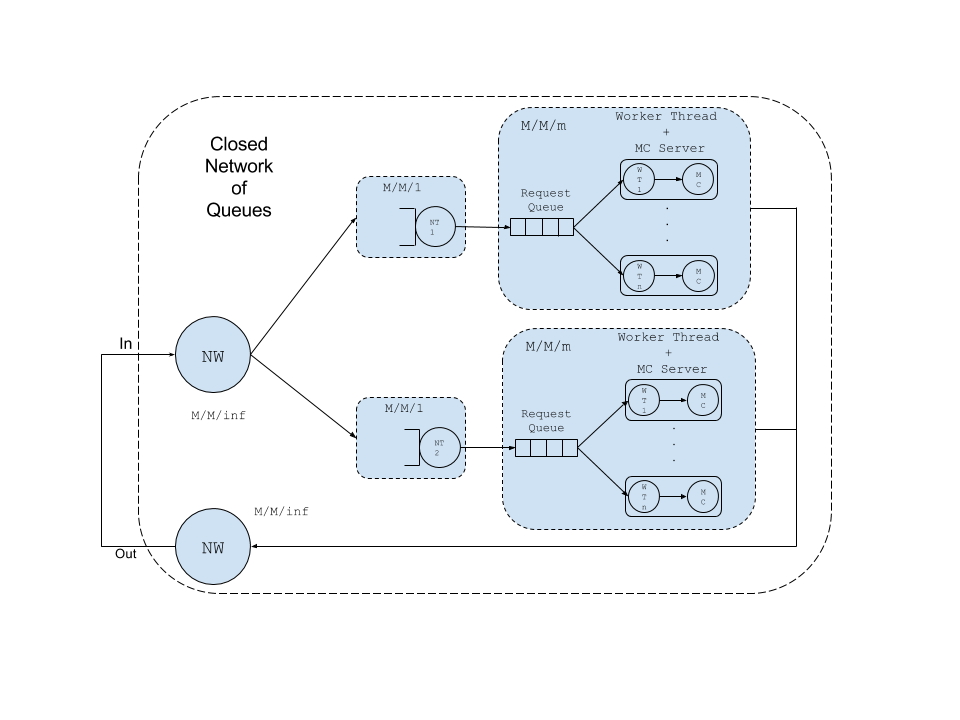
\includegraphics[scale=0.5]{images/7_network_of_queues}
\caption{Network of Queues Model of the system}
\label{fig:32_network_of_queues}
\end{figure}

\subsubsection{Parameters of the Model}


\pagebreak
\appendix
\section{General Notes on Experimental Setup} \label{appendix_a}
Before we delve into the experimental details and analysis of each of the following sections, there are a few common things to keep in mind about how the experiments are conducted. These are presented here in order to avoid repeating them in each subsequent section and to keep them in mind while explaining the outcomes of our experiments. The scripts used to run the experiments can be found at \texttt{scripts/1\_exp\_runners} directory. We have one script per section (of analysis in the report). Note that, unless stated otherwise, each configuration is repeated three time to remove random fluctuations of the observed values. Finally, all middleware and memcached instances listen on port \underline{6969}

\paragraph{Abbreviations}
For the sake of brevity, we use several abbreviations throughout the report. Most can be inferred from context, nevertheless, here are a few abbreviations we use.
\begin{itemize}
	\setlength{\itemsep}{0pt}
	\setlength{\parskip}{0pt}
	\setlength{\parsep}{0pt}
	\item MT Memtier Instance if more than one memtier per VM, else load generating VM itself
	\item LG Load Generating VMs, these are A2 VMs
	\item MW Middleware, these are A4 VMs
	\item MC Memcached servers / VMs, these are A1 VMs
	\item TPS Throughput
	\item LAT / RT Latency / Response Time (used interchangeably)
\end{itemize}


\subsection{VM Allocation and Deallocation}
We have split up the automated running of experiments for each of the sections into separate scripts. Each of the scripts contains calls to the Azure Command Line Utility which allocates the Virtual Machines needed for the experiments(we use the command \texttt{az vm allocate} to allocate and start VMs). Once this is done, memcached instances are started on the A1 VMs, appropriate directories to store the logs are created on the A2 and A4 VMs (the load generating and middleware VMs). Finally, the memcached servers are pre-populated as discussed in a subsequent section. And before running the different configurations, ping tests are run to ensure stable network conditions, this is discussed in the next section. Finally, once all the experiments are done, the scripts deallocate the VMs (using \texttt{az vm deallocate}) so that we don't waste credits keeping the VMs running when not in use. 

This way, we ensure that all the numbers we report in a given section are from similar if not same network conditions and thus the numbers can be compared and system behaviours can be inferred from it.

\subsection{Network Latencies}
In order to make sure that the network connections between the different components of a setup are similar, we run pings between each individual connections between components of our setup the before starting our experiments. Depending on the experiment in question, the setup can vary. For example, 1, 2 or 3 Load generating VMs with one or two \texttt{memtier\_benchmark} instances per VM connected to one or two middlewares each in turn can be connected one, two or three memcached servers. The results of these ping tests can be found in \texttt{logs/<EXP\_NAME>/mt\_log/} directories each with the prefix \texttt{ping}. It can be argued that the network latencies and general behaviour can vary depending on the amount of load you put on the network due to the TCP Flow Control mechanisms kicking in to avoid congestion. This means that raw mean latencies from these pings should be considered with the grain of salt. We observe that the mean latencies, as measured by ping (the exact command used is \texttt{ping -c 5 <private\_IP\_of\_destination}) have the same order of magnitude (a few milliseconds) across all experiments. On a closer look at the exact numbers, some of the links can have almost double the mean latency of another link. For example, see \texttt{ping\_foraslvms1.txt} and \texttt{ping\_foraslvms2.txt} at \texttt{logs/2a\_one\_server\_base\_line\_log}. The former has more than double the average latency of the latter. Though, this may not cause significant issues as we usually average the latencies across the load generating VMs, it is important to note this observation as a plausible source of deviations from the norm. 


\subsection{Pre-populating memcached servers}
After starting the memcached instances, they are empty. This means that any GET request will return an empty response (just a \texttt{END\textbackslash r\textbackslash n}). These are cheap to construct and send back and thus can have significant effects in the numbers we measure if we have "GET Misses". In order to avoid these, we always pre-populated the memcached servers using memtier instances to ensure that there are no misses. We do this even when there are only write-only workloads, in order to ensure that we are comparing similarly loaded memcached servers across different workloads (read-only, write-only, 50-50). We use the following command to prepopulate the MC servers. We use very long expiry range in order to make sure that no keys are evicted before the experiments are completed. \\

\texttt{memtier\_benchmark -s <PRIVATE\_MC\_IP> -p <MC\_PORT> -P memcache\_text -n allkeys} \\
\texttt{ --ratio 1:0 --key-maximum 10000 --hide-histogram --expiry-range 99999-100000} \\
\texttt{ -d 1024 --key-pattern=S:S> /dev/null 2>\&1}

\subsection{Performance Monitoring (\texttt{dstat})}
In many of the analysis that we subsequently do, two key questions we try to answers are what is the bottleneck of the system and what are the utilizations of the different components. We hope to get these purely from the MT and MW logs. However, since the memtier instances are running on mediocrely powerful VMs, we can get more insights by looking at how much the CPU, RAM and Network interface are used. This will allow us to better explain why a component is a bottleneck or not. We use \texttt{dstat} on the LG VMs for this purpose and save the results in a CSV file in the same directory as the memtier logs. These files start with the prefix \texttt{dstat\_}. The exact command we use is \texttt{dstat -cmn --nocolor --output <out\_file> 5 18 >/dev/null </dev/null 2>\&1}. Here the readings are taken every 5 seconds and are done 18 times (roughly the same amount of time a single repetition of a configuration runs)

\subsection{Experimental Startup}
All experiments for a section are done together and the VMs and deallocated only after all the experiments belonging to one section are completed. In each of the experiments and each of the repetitions we run, we do the following steps. 
	\begin{itemize}
	\setlength{\itemsep}{0pt}
	\setlength{\parskip}{0pt}
	\setlength{\parsep}{0pt}
	\item Start the MC instances
	\item create log directories in MT and MW instances
	\item Pre-populate the MC servers
	\item Start Middlewares (if any are needed)
	\item Wait 20 seconds for Middleware to connect to all the memcached servers to avoids errors
	\item Start \texttt{dstat}
	\item Run the \texttt{memtier\textunderscore benchmark}(s)
	\item Kill the Middleware
	\item Wait for 5 seconds before starting next repetition / configuration
\end{itemize}

\subsection{Common Configurations}
\subsubsection{Memcached}
All instances of memcached across all experiments are started with this command \texttt{memcached -t 1 -p 6969}. We always run the servers in single threaded mode because the A1 VMs have only one core and also because it is advisable to use memcached in single-threaded mode.

\subsubsection{Memtier}
Many of the flags that we use with memtier depend on the experiment in question but there are a few that are common across all experiments. An incomplete set is \texttt{memtier\_benchmark -s <Dest\_IP> -p 6969 -P memcache\_text --test-time 80 --key-maximum 10000 -d 1024 \\
	--json-out-file <JSON\_FILE\_NAME>}. The additional  flags used in each report will be described in their corresponding sections.

\end{document}
\grid
